\documentclass[conference]{IEEEtran}
\IEEEoverridecommandlockouts
% The preceding line is only needed to identify funding in the first footnote. If that is unneeded, please comment it out.
\usepackage{cite}
\usepackage{amsmath,amssymb,amsfonts}
\usepackage{algorithmic}
\usepackage{graphicx}
\graphicspath{{figures/}}   % 그림은 모두 figures/ 아래에 둔다

% --- float 배치 완화 ---------------------------------------------------
% 두 단 폭 float(figure*/table*)은 페이지 맨 위에만 놓일 수 있어서, 기본값으로는
% 자기 절을 지나 뒤로 밀린다. 한 페이지가 float 에 내줄 수 있는 몫을 늘려
% 각 그림/표가 자기 절 안에 앉도록 한다.
\renewcommand{\topfraction}{0.92}        % 페이지 위쪽 float 최대 비율 (기본 0.7)
\renewcommand{\bottomfraction}{0.75}     % 아래쪽 (기본 0.3)
\renewcommand{\textfraction}{0.06}       % 본문이 차지해야 하는 최소 비율 (기본 0.2)
\renewcommand{\floatpagefraction}{0.72}  % float 전용 페이지 판정 문턱 (기본 0.5)
\renewcommand{\dbltopfraction}{0.92}     % 두 단 폭 float 의 위쪽 몫 (기본 0.7)
\renewcommand{\dblfloatpagefraction}{0.72}
\setcounter{topnumber}{3}                % 페이지 위쪽 float 개수 (기본 2)
\setcounter{bottomnumber}{2}
\setcounter{totalnumber}{5}              % 한 페이지 총 float 개수 (기본 3)
\setcounter{dbltopnumber}{3}
% ----------------------------------------------------------------------
\usepackage{textcomp}
\usepackage{xcolor}
\usepackage{multirow}
\usepackage{booktabs}   % tables/*.tex 가 \toprule/\midrule/\cmidrule/\bottomrule 를 쓴다
\usepackage{tikz}       % Fig.2 (영공간 도식) 가 쓴다
\usetikzlibrary{arrows.meta,positioning,calc}
\usepackage[hidelinks]{hyperref}
\usepackage{kotex}   % 한글 주석/메모용. 한글을 쓰지 않으면 주석 처리해도 됨
\newcommand{\rev}[1]{\textcolor{red}{#1}}
%수정한 부분을 빨간색으로 표시함
\newcommand{\NA}{\text{--}}   % tables/table2_baselines.tex 이 쓰던 미정의 매크로
\newcommand{\Pending}{\rev{--}}   % tables/table_main_v2.tex 이 쓰는데 정의가 없었다 (실물 대기 칸)

% --- Method 절의 정리 환경 (3_method.tex 이 씀) --------------------------
% IEEEtran 은 IEEEproof 는 주지만 theorem 계열은 직접 선언해야 한다.
\newtheorem{lemma}{Lemma}
\newtheorem{proposition}{Proposition}
\newtheorem{corollary}{Corollary}
\newtheorem{remark}{Remark}
% ------------------------------------------------------------------------

\def\BibTeX{{\rm B\kern-.05em{\sc i\kern-.025em b}\kern-.08em
    T\kern-.1667em\lower.7ex\hbox{E}\kern-.125emX}}
% 분량 맞춤: raggedbottom 은 단 아래를 매 페이지 비워 두므로 flushbottom 으로
% 되돌리고, float 주변 간격을 IEEE 기본보다 조금 좁힌다 (내용 삭제 없는 압축).
\setlength{\textfloatsep}{8pt plus 2pt minus 4pt}
\setlength{\dbltextfloatsep}{8pt plus 2pt minus 4pt}
\setlength{\floatsep}{6pt plus 2pt minus 2pt}
\setlength{\dblfloatsep}{6pt plus 2pt minus 2pt}
\begin{document}

\title{PIVoT: Part-Wise Identification of Volume-Aware Density via Multi-Topology Reorientation}


\author{Jun Hyeok Lee\textsuperscript{*}, Yu Seong Cheon\textsuperscript{*}, Sang Woo Han\textsuperscript{*}, and Yong Seok Lee\textsuperscript{$\dagger$}}

\maketitle

\begin{abstract}
Reproducing articulated objects faithfully in simulation is essential for learning robotic manipulation, and an object's physical behavior is determined by each part's volume and density, so both must be identified at the part level. Existing vision-based methods, however, estimate volume only at the whole-object level and infer density from appearance alone, while interaction-based identification has been applied only to rigid bodies; the design of measurement poses and paths for identifying the part-wise parameters of an articulated object has not been addressed. We present PIVoT, a closed-loop pipeline that identifies the per-part density of articulated objects through active robot interaction and produces sim-ready assets faithful in appearance, geometry, and physics. Based on information gain, PIVoT suggests to the user joint configurations that minimize the null space of the density estimate; at each configuration, the robot collects wrench data along collision-free paths through three measurement poses under different gravity directions and updates the per-part densities until their uncertainty converges. User intervention beyond reconstruction is limited to adjusting the object to the suggested joint configuration, and the per-part volumes on which the identification rests are corrected by multi-view-consistency-based mesh refinement and per-part scaling. With a single RGB-D camera and a 6-DoF arm, we validate PIVoT in simulation on three real articulated objects, including two custom objects with per-part ground-truth density\rev{; validation on a fourth object (laptop) and on the physical robot is in preparation}.
% [번역] 시뮬레이션에서 articulated object 를 충실하게 재현하는 것은 로봇
%   조작 학습에 필수적이며, 물체의 물리적 거동은 part 별 부피와 밀도로
%   결정되므로 이 둘을 part 단위로 식별해야 한다. 그러나 기존 vision 기반
%   방법은 부피를 물체 전체 단위로만 추정하고 밀도는 외형만으로 추정하며,
%   상호작용 기반 식별은 rigid body 에만 적용되어 왔다. 관절체의 part 별
%   parameter 를 식별하기 위한 측정 자세와 경로 설계는 다루어지지 않았다.
%   본 연구에서는 active robot interaction 으로 articulated object 의 part
%   별 밀도를 식별하여 외형·기하·물성에 모두 충실한 sim-ready asset 을
%   생성하는 closed-loop pipeline 인 PIVoT 를 제안한다. PIVoT 는
%   information gain 에 기반해 밀도 추정의 null space 를 최소화하는 joint
%   configuration 을 사용자에게 제시하고, 각 configuration 에서 서로 다른
%   중력 방향의 측정 자세 3개를 collision-free 경로로 이동하며 렌치를
%   수집하고, 불확실성이 수렴할 때까지 part 별 밀도를 갱신한다. 재구성 이후
%   추가되는 사용자 개입은 제시된 joint configuration 조정으로 제한되며,
%   밀도 식별의 기반이 되는 part 별 부피는 multi-view consistency 기반 mesh
%   refinement 와 part 별 scaling 으로 보정된다. 단일 RGB-D 카메라와 6-DoF
%   arm 환경의 시뮬레이션에서, part 별 GT 밀도를 가진 커스텀 물체 둘을
%   포함한 실제 관절체 3종에 대해 검증한다(4번째 물체(노트북)와 실물 로봇
%   검증은 준비 중 — \rev{} 표시).
\end{abstract}

\begin{IEEEkeywords}
Articulated object, Physical property identification, Real2Sim
\end{IEEEkeywords}

\section{Introduction}

Physics simulation has become a driving force in robotic manipulation, letting policies be trained and evaluated before real-world deployment. The real world is full of portable articulated objects---laptops, foldable phones, desk lamp stands---whose friction-holding joints keep their configuration unless a force is deliberately applied. For simulation with such objects to transfer, sim-ready assets must be dynamically as well as visually and kinematically faithful; hand-building them does not scale \cite{pfaff2025scalable}, motivating real-to-sim pipelines that construct them from real observations.
% [번역] 물리 시뮬레이션은 로봇 조작 연구의 핵심 동력이 되어, 정책을 실기
%   배포 전에 학습·평가할 수 있게 한다. 실세계에는 노트북, 폴더블폰, 책상용
%   스탠드처럼 마찰 유지 관절 덕분에 힘을 일부러 주지 않는 한 형상이
%   보존되는 휴대용 관절 물체가 많다. 이런 물체의 시뮬레이션 결과가
%   전이되려면 sim-ready asset 이 외형·운동학뿐 아니라 동역학까지 충실해야
%   하는데, 손으로 만드는 일은 느리고 확장되지 않아 실세계 관측에서 asset 을
%   직접 구축하는 real-to-sim 파이프라인이 이어져 왔다.

% ---------------------------------------------------------------------------
% ---------------------------------------------------------------------------
\begin{figure}[t]
\centering
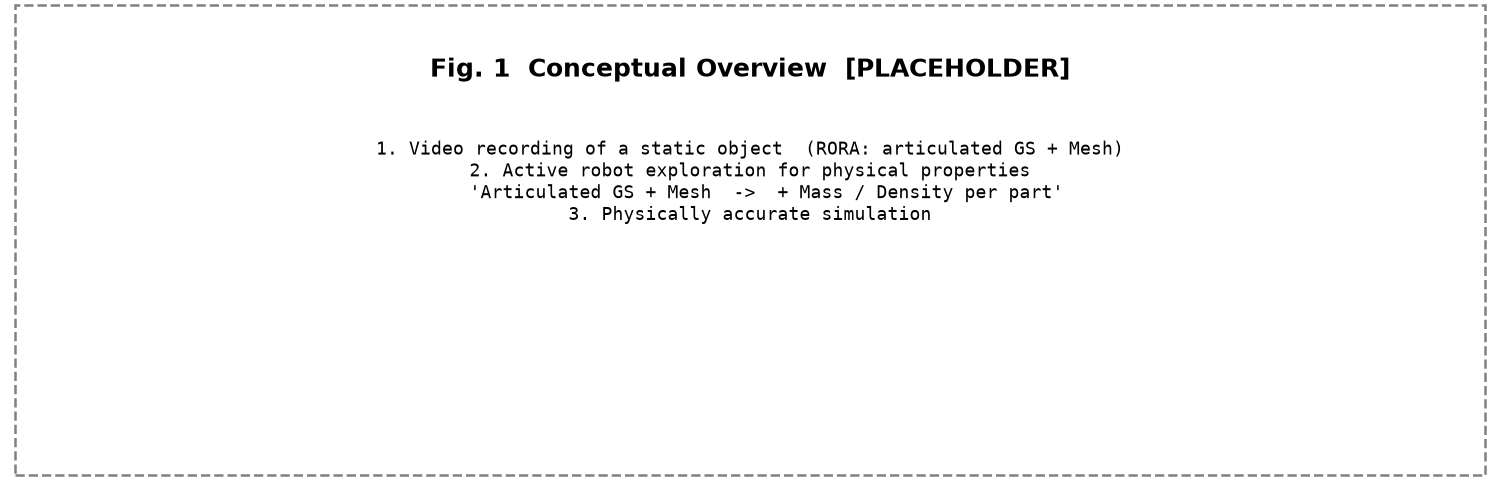
\includegraphics[width=\linewidth]{fig1.png}
\caption{PIVoT overview. (1)~Video of a static object yields an articulated
reconstruction; (2)~robot reorientation under different gravity directions
adds per-part mass and density; (3)~the asset reproduces the object's behavior
in simulation.}
% [번역] PIVoT 개관. (1) 정적 물체 영상에서 관절 재구성을 얻고, (2) 서로 다른 중력 방향의 로봇 재배향이 part 별 질량·
%   밀도를 더하며, (3) asset 은 물체의 거동을 시뮬레이션에서 재현한다.
%   ("사용자는 제시된 joint configuration 조정만" 은 초록·III·IV-E 산문에.)
% [메모] Fig. 1 — Teaser. fig1.png 은 자리표시용이다. v2 사양(가이드라인
%   [Figure 1: Conceptual Overview], 번호형 콜라주 3단계):
%   1. Video recording of a static object — 비디오 입력. RORA 결과물
%      (articulated GS + Mesh)을 작은 중간 결과로 표시하여 출발점임을 보여줌.
%   2. Active robot exploration for physical properties — 로봇 팔이 물체를
%      서로 다른 방향으로 기울여 들고 있는 장면 + 사용자가 joint
%      configuration 을 바꾸는 작은 아이콘. 화살표 라벨:
%      "Articulated GS + Mesh -> + Mass / Density per part".
%   3. Physically accurate simulation — 무게중심·관성에 따른 물체 거동
%      (기울어짐, 낙하 등)이 실제와 일치하는 장면.
\label{fig:teaser}
\end{figure}

Recent 3D Gaussian Splatting (3DGS) pipelines recover an articulated object's appearance, part-level meshes, and joint structure up to a URDF \cite{lee2026rora}. Dynamically faithful simulation additionally requires each part's mass, center of mass, and rotational inertia, all of which follow from per-part geometry and density. Reconstruction supplies the geometry; density is precisely what a camera cannot observe, since identical-looking parts can hide entirely different mass distributions. Existing pipelines therefore guess density---from appearance, material priors, or a generative model \cite{shuai2025pugs,chopra2026physgs,cao2026physxomni}---while methods that measure mass through real interaction keep the object rigid \cite{pfaff2025scalable,nadeau2023sum}. To our knowledge, no prior work has identified, from wrist force/torque measurements, the density of the links themselves for an articulated object in which two or more links carry independently unknown mass: interaction-based attempts on articulated objects have estimated link masses from vision rather than force sensing, and force-based identification has been demonstrated only on mechanisms with a single movable link \cite{he2027rigpi}.
% [번역] 최근의 3D Gaussian Splatting(3DGS) 파이프라인은 관절 물체의 외형,
%   part 단위 mesh, 관절 구조를 URDF 수준까지 복원한다. 동역학까지 충실한
%   시뮬레이션에는 각 part 의 질량·무게중심·회전관성이 추가로 필요한데, 이
%   셋은 모두 part 별 형상과 밀도에서 따라 나온다. 형상은 재구성이 주지만,
%   밀도는 정확히 카메라가 볼 수 없는 것이다. 겉모습이 같은 부위가 전혀 다른
%   질량 분포를 숨길 수 있기 때문이다. 그래서 기존 파이프라인은 밀도를
%   외형·재질 사전지식·생성 모델로 추측하고, 실제 상호작용으로 질량을 재는
%   방법들은 물체를 강체로 두어 왔다. 우리가 아는 한, 손목 force/torque
%   측정에 근거하여, 독립적으로 미지인 질량을 가진 링크가 2개 이상인 관절체의
%   링크 자체 밀도를 식별한 연구는 없다. 관절체를 다룬 상호작용 기반 시도는
%   힘이 아니라 비전으로 링크 질량을 추정했고, 힘 기반 식별은 움직이는 링크가
%   하나뿐인 기구에서만 실증되었다.

The gap persists not because the rigid-body methods are weak, but because the measurement they rely on saturates. A quasi-static wrench constrains only the zeroth and first mass moments: for an object with $P$ parts a single joint configuration determines at most $1+\min(3,P)$ independent density combinations---at most four---however the wrist reorients the object. Changing the object's own joint configuration is therefore the only mechanism that brings the remaining combinations into view, and the same analysis yields a lower bound on the number of configurations required, computable from geometry alone, before any wrench is measured.
% [번역] 이 공백이 남은 것은 강체 방법들이 약해서가 아니라, 그들이 의존하는
%   측정 자체가 포화하기 때문이다. 준정적 렌치는 0차·1차 질량 모멘트만
%   구속하므로, part 가 P 개인 물체에서 단일 관절 형상은 손목이 물체를 어떻게
%   재배향하든 최대 1+min(3,P) 개, 즉 많아야 네 개의 독립 밀도 조합만
%   결정한다. 따라서 나머지 조합을 보이게 만드는 유일한 수단은 물체 자신의
%   관절 형상을 바꾸는 것이고, 같은 분석에서 필요한 관절 형상 개수의 하한이
%   나온다 — 렌치를 하나도 재기 전에 물체의 형상 정보만으로 계산된다.

Turning this into a working system requires two ingredients the rigid-body literature never needed. The first is choosing \emph{which} configurations to measure: only a handful are affordable, so each should maximize expected information gain about the per-part densities. The second is physically \emph{reaching} the measurement poses: each configuration is measured under three gravity directions, and the robot must carry the grasped object between poses without collision and without overloading its joints, across topologies whose geometry---hence collision constraints---differ. Moreover, the joint configuration is read by a camera rather than commanded, so the design variable itself carries error; a total-least-squares formulation absorbs it, and conditioning---not the rank condition---sets the practical limit.
% [번역] 이를 동작하는 시스템으로 만들려면 강체 식별 문헌에는 필요 없던 두
%   요소가 필요하다. 첫째는 '어느' 형상을 측정할지 고르는 일이다. 감당할 수
%   있는 형상 수가 몇 개뿐이므로, 각 형상은 part 별 밀도에 대한 기대
%   정보이득을 최대화해야 한다. 둘째는 측정 자세에 물리적으로 '도달'하는
%   일이다. 각 형상은 중력 방향 3개에서 측정하고, 로봇은 잡은 물체를 자세
%   사이로 옮기는 동안 자기 자신·환경과 충돌하지 않고 물체의 관절에 무리를
%   주지 않아야 한다 — 기하 형상이, 따라서 충돌 제약이 달라지는 topology 들에
%   걸쳐서. 나아가 관절 형상은 명령한 값이 아니라 카메라가 읽은 값이므로 설계
%   변수 자체가 오차를 갖는다. 총최소제곱 정식화가 이를 흡수하며, 실질적
%   한계를 정하는 것은 rank 조건이 아니라 조건수다.

We therefore propose PIVoT (Fig.~\ref{fig:teaser}), a closed-loop pipeline that identifies the per-part density of portable articulated objects through active robot interaction, turning the part-level reconstruction of \cite{lee2026rora} into a sim-ready asset faithful in appearance, geometry, and physics. The reconstruction-stage intervention is inherited from \cite{lee2026rora}; the additional intervention for physics estimation is one adjustment of the object to the suggested joint configuration. Our contributions are:
% [번역] 그래서 우리는 active robot interaction 으로 휴대용 관절 물체의
%   part 별 밀도를 식별하여, [RORA] 의 part 단위 재구성을 외형·기하·물성에
%   모두 충실한 sim-ready asset 으로 만드는 폐루프 파이프라인 PIVoT 를
%   제안한다(그림 1). 재구성 단계의 개입은 [RORA] 와 동일하게 상속되며, 물성
%   추정을 위해 추가되는 개입은 제시된 관절 형상으로 물체를 조정하는 한
%   번뿐이다. 본 논문의 기여는 다음과 같다.

\begin{itemize}
    \item \textbf{Information-theoretic part-wise density identification:} a
    lower bound on the number of joint configurations as a function of the part
    count, selection by expected information gain, and an uncertainty-aware
    per-part density update.
% [번역] (1) 정보이론적 part 별 밀도 식별 — part 수의 함수인 관절 형상 개수의
%   이론적 하한, 기대 정보이득에 의한 형상 선택, 상호작용 데이터로부터의
%   불확실성 기반 part 별 밀도 갱신.

    \item \textbf{Multi-topology measurement path design:} three measurement
    poses under different gravity directions per configuration, linked by
    RRT-planned collision-free paths that account for object geometry,
    self-collision, and obstacles across topologies.
% [번역] (2) multi-topology 측정 경로 설계 — 관절 형상마다 서로 다른 중력
%   방향의 측정 자세 3개를 정의하고, topology 에 걸쳐 물체 기하·self-collision·
%   장애물을 고려하는 RRT 기반 planner 로 그 사이 collision-free 경로를 생성.

    \item \textbf{Closed-loop sim-ready asset pipeline:} mesh refinement
    and per-part scaling reduce volume error, and the components above integrate
    into a pipeline limiting additional user intervention to one
    joint-configuration adjustment, validated in
    simulation on three articulated objects, two with per-part ground-truth
    density\rev{; validation on a fourth object (laptop) and on the physical
    robot is in preparation}.
% [번역] (3) 폐루프 sim-ready asset 파이프라인 — part 별 부피 오차를 줄이는
%   mesh refinement 와 scaling 위에 위 요소들을 통합하여 추가 사용자 개입을
%   관절 형상 조정 한 번으로 제한하며, part 별 GT 밀도를 가진 커스텀 물체 둘을
%   포함한 관절체 3종의 시뮬레이션으로 검증한다(4번째 물체(노트북)와 실물
%   로봇 검증은 준비 중 — \rev{} 표시).
\end{itemize}

%%%%%%%%%%%%%%%%%%%%%%%%%%%%%%%%%%%%%%%%%%%%%%%%%%%%%%%%%%%%%%%%
% [메모] 8/30 3차 개정 (WRITING_BRIEF.md §7 · paper guideline v2 기준).
%   소절 4개 -> 3개 (가이드라인 v2 의 3분류). A: sim-ready 재구성 (RORA/ArtVIP/
%   JODA + 기하·관절 전용 계보). B: vision 물성 추정 — 부피/밀도를 나누어 서술,
%   "실측과 접점이 전혀 없다" 는 과장 제거 (실측은 평가 GT 로만 들어옴을 명시,
%   §7.2). C: interaction 물성 추정 — (i) 단일 강체 실조작 (Nadeau 의 "part" 가
%   강체 내부 재질 영역임을 명시), (ii) 다자세 정지 렌치 표준 결과 (특정 논문에
%   귀속시키지 않음, §7.3), (iii) 최근접 선행연구 구분: Kumar 2019 신규 인용
%   (비전/비파지 푸시/이산 분류 — 3가지 차이 한 문장), RigPI 는 실물 검증 물체가
%   가동 링크 1개뿐임을 명시, 주장은 §7.4 의 3축 문구로 좁힘. 구 C(고전 분석)·
%   D(여기·능동 탐색) 소절은 C 말미 한 문단으로 압축 (Gautier & Khalil, Swevers,
%   RPNA, ASID 유지; Hausman 은 C(iii) 로 이동; hausman2015active 와
%   memmel2024asid 는 별개 논문으로 분리 서술, §7.5).
% [메모] 8/30 8-페이지 압축: 인용 11건 제거 (CUTS.md 참조) — mayeda1990base,
%   lee2020geometric, lee2021optimal, janot2014instrumental, jin2025ugraph,
%   eppner2018physics, zhai2024nerf2physics, xu2025gaussianproperty,
%   kim2025screwsplat, lee2026artsplat, li2026uniphysgen. 신규 bib 키:
%   artvip2026, joda2026, jiang2022ditto, liu2023paris, mandi2024real2code,
%   artgs2025, cao2025physx3d, kumar2019estimating, nadeau2022fast,
%   activetactile2023, kubus2008online. le2026siphy 는 ECCV 2026 로 정정.
% [메모] 8/30 압축 개정: 8/27·8/20 구 판본 주석 블록은 삭제했다 (git 과 v1
%   트리에 보존되어 있음).

\section{Related Work}

\subsection{Sim-Ready Reconstruction of Articulated Objects}

Articulated-object reconstruction recovers appearance, part decomposition, and
kinematics from interaction or images
\cite{jiang2022ditto}.
RORA, our starting point, exports part-bound Gaussians, part meshes, and a
URDF from a single-configuration video through human-in-the-loop joint
proposals \cite{lee2026rora}. ArtVIP's assets are billed as physically
faithful but hand-authored, not identified from measurements of the simulated
instance \cite{artvip2026}; JODA infers joint dynamics---friction, damping,
detents---with a VLM, leaving link masses unaddressed \cite{joda2026}. The lineage delivers visual and
geometric fidelity but no measured physics; we take such a reconstruction as
input and add physics by measurement.
% [번역] 관절 물체 재구성은 상호작용이나 영상으로부터 외형, 부위 분할, 기구학
%   구조를 복원한다. RORA 는 단일 정적 형상 영상에서 human-in-the-loop 관절
%   제안을 거쳐 part 결합 Gaussian, part mesh, URDF 를 내보내며 본
%   파이프라인의 출발점이다. ArtVIP 는 물리적 충실도를 표방하는 관절 자산을
%   제공하지만 전문 모델러의 수작업 저작이지 시뮬레이션 대상 개체의 실측 기반
%   식별이 아니고, JODA 는 관절 동역학(마찰·댐핑·디텐트)을 VLM 으로 추론할 뿐
%   링크 질량은 다루지 않는다. 이 계보는 시각·기하 충실도를 주지만 시뮬레이션
%   거동을 결정하는 물성은 없거나 수작업이다. 본 연구는 그런 재구성을
%   입력으로 받아 빠진 물리를 측정으로 채운다.

\subsection{Vision-Based Physical Property Estimation}

Vision-based methods estimate properties without contact. For \emph{volume},
PUGS integrates a Gaussian-splatting reconstruction's volume to predict object
mass \cite{shuai2025pugs}, and the PhysX series uses its
generated meshes' volume
\cite{cao2026physxomni}.
Volume thus enters at whole-object granularity or via generated geometry; an individual part---thin, hollow, or occluded---retains a large
error.
% [번역] 시각 기반 방법들은 접촉 없이 물성을 추정한다. 부피 쪽에서 PUGS 는
%   Gaussian splatting 재구성의 부피를 적분해 물체 질량을 예측하고, PhysX
%   계열과 UniPhysGen 은 자신이 생성한 mesh 의 부피를 그대로 쓴다. 부피가
%   물체 전체 단위로 들어오거나 생성된 기하에서 상속되므로, 얇거나 속이
%   비었거나 가려진 개별 part 의 부피 오차는 크게 남는다.

For \emph{density}, the generative series looks up a material database given a
predicted material class, while PhysGS and part-level SiPhy infer it from
appearance and language-derived priors
\cite{chopra2026physgs,le2026siphy}.
These estimates are grounded only in appearance priors: real measurements enter
as evaluation ground truth---never as an input. Appearance does
not determine density; we identify it by measurement instead.
% [번역] 밀도 쪽에서 같은 생성 계열은 예측된 재질 클래스로 재질 DB 에서 값을
%   조회하고, NeRF2Physics, GaussianProperty, PhysGS, part 단위의 SiPhy 는
%   외형과 언어 유래 사전지식으로 추론한다. 이들 추정은 외형 사전지식에만
%   근거한다. 실측은 평가용 GT 로는 들어오지만 추정의 입력으로는 결코 들어오지
%   않는다. 외형이 밀도를 결정하지 않으므로 그 값은 해당 개체에 대해 신뢰할 수
%   없고, 우리는 측정으로 식별한다.

\subsection{Interaction-Based Physical Property Estimation}

Interaction-based methods measure, but on single rigid bodies: quasi-static
wrenches identify masses of homogeneous material regions inside one
body---the ``parts'' of \cite{nadeau2023sum} are such regions, not articulated
links---inertial parameters are identified during pick-and-place
\cite{nadeau2022fast}, and Scalable Real2Sim generates
assets with physically feasible inertial parameters from robot sensing
\cite{pfaff2025scalable}.
% [번역] 상호작용 기반 방법들은 실제로 측정하지만 단일 강체가 대상이다. 정지
%   렌치로 한 강체 내부의 균질 재질 영역별 질량을 식별하는데 —
%   \cite{nadeau2023sum} 의 "part" 는 그런 영역이지 관절로 연결된 링크가
%   아니다 — pick-and-place 중 관성 파라미터를 식별하거나, Scalable Real2Sim
%   처럼 로봇 센싱으로 물리적으로 실현 가능한 관성 파라미터의 asset 을
%   생성한다.

A second thread reorients a grasped rigid body, reading the static wrench: one
gravity direction fixes mass, two non-parallel add the center of mass, a
non-coplanar third separates sensor bias; the inertia tensor
produces no quasi-static wrench and classically requires dynamic trajectories
\cite{atkeson1986estimation,kubus2008online} (cf.\ Sec.~\ref{sec:theory}).
% [번역] 두 번째 갈래는 파지한 강체를 재배향하며 정지 렌치를 읽는다. 중력
%   방향 하나면 질량이, 비평행 두 방향이면 무게중심까지 정해지고, 비공면 세
%   번째는 센서 바이어스를 분리한다. 관성 텐서는 준정적 렌치를 전혀 만들지
%   않아 고전적으로 동적 궤적을 요구한다(III 절 참조).

The closest prior work is Kumar et al.~\cite{kumar2019estimating}, which
estimates per-link mass of two- and three-link objects on a real UR10; it
differs in sensing with vision (an RGB-D camera and per-link
markers) rather than force--torque, in pushing the object non-prehensilely
rather than grasping and reorienting it, and in classifying among five discrete
mass-distribution hypotheses rather than regressing continuous values. RigPI
identifies parameters via VLM-seeded differentiable simulation with
force--torque sensing \cite{he2027rigpi}, but its real-robot validation
objects each have only one moving link; its multi-link results remain in
simulation. Interactive perception
acts on articulated objects but estimates the kinematic model---joint axes
and types---not link masses or densities
\cite{hausman2015active}. To our knowledge, no prior work
identifies, from wrist force--torque measurements, the densities of two or more
independently unknown links within one mechanism.
% [번역] 가장 가까운 선행연구는 Kumar 등으로, 실물 UR10 에서 2·3링크 관절체의
%   링크별 질량을 추정한다. 그러나 F/T 가 아니라 비전(RGB-D 카메라와 링크별
%   마커)으로 센싱하고, 파지·재배향이 아니라 비파지 밀기를 쓰며, 연속 회귀가
%   아니라 다섯 개의 이산 질량분포 가설 중 분류를 한다는 세 가지 점에서 본
%   연구와 다르다. RigPI 는 F/T 센싱과 VLM 초기화 미분 가능 시뮬레이션으로
%   파라미터를 식별하지만, 실물 검증 물체는 각각
%   움직이는 링크가 하나뿐이고 다중 링크 결과는 시뮬레이션에 그친다.
%   interactive perception 은 관절 물체를 능동 조작하지만 목적은 관절 축·타입,
%   즉 kinematic model 추정이지 링크의 질량·밀도가 아니다. 우리가 아는 한,
%   손목 F/T 실측으로 하나의 기구 안에서 독립적으로 미지인 링크 2개 이상의
%   밀도를 식별한 연구는 없다.

Our design machinery is classical: base-parameter analysis delimits
which inertial combinations any regressor can resolve
\cite{wensing2024geometric}; Gautier--Khalil
and Swevers et al.\ condition the regressor by optimizing
identification trajectories
\cite{gautier1992exciting,swevers1997optimal}; ASID brings the same logic to
learned exploration policies maximizing Fisher information
\cite{memmel2024asid}. All design an actuated robot's trajectory, its
configuration read by encoders; PIVoT instead designs, in a closed loop, a
passive object's joint configuration and the gravity directions under which
it is reoriented.
% [번역] 우리가 딛고 서는 설계 도구는 고전적이다. base parameter 분석은 어떤
%   회귀 행렬이든 분해할 수 있는 관성 조합을 한정하고, Gautier-Khalil 과
%   Swevers 등은 동적 식별 주행의 궤적을 최적화해 회귀 행렬의 조건을 좋게
%   하며, ASID 는 같은 논리를 Fisher 정보를 최대화하는 학습된 탐색 정책으로
%   가져간다. 모두 엔코더로 형상을 읽는 구동 로봇의 궤적을 설계한다. PIVoT 는
%   반대로 수동 물체의 관절 형상과 재배향할 중력 방향들을 폐루프로 설계한다.

%%%%%%%%%%%%%%%%%%%%%%%%%%%%%%%%%%%%%%%%%%%%%%%%%%%%%%%%%%%%%%%%
% [메모] 8/30 5차: COMPRESSION_RULES.md 에 따라 3,556 단어에서 압축
%   (4차 개정의 소절 구조 A~E 와 정리 환경 8개·라벨·\rev 전부 보존).
%   증명 처리: 보조정리 1 은 한 문장. 명제 1(rank 천장)·명제 3(라운드 하한)
%   증명은 표준 단계(PSD 순서·rank 준가법성·그람 행렬)라 진술 뒤 한 구절로
%   강등. 명제 2 증명은 짧아 유지. 측정 방향 수확체감 수치열
%   (12.88/25.41/26.35/26.92/27.73 nat, 2.72배)은 4_exp 의 Table IV(tab:path)
%   가 이미 실으므로 본문에는 "삼면체=무릎" 형태와 0.0 % / -39.9 %
%   (1.031 -> 0.620 N·m) 만 유지. Wensing/base-parameter 대비 문단은
%   2_relwork 가 같은 인용을 다루므로 한 문장으로 축약. 삭제 산문은 CUTS.md.
%%%%%%%%%%%%%%%%%%%%%%%%%%%%%%%%%%%%%%%%%%%%%%%%%%%%%%%%%%%%%%%%

\section{Method}

\subsection{Problem Formulation and Overview}
\label{sec:formulation}

% ---------------------------------------------------------------------------
% Fig. 2 — Overall pipeline.  가이드라인 v2 의 [Figure 2] 사양을 그대로 옮긴다.
%   위층 Offline (회색, 직선 흐름):
%     (a) Articulated reconstruction — RORA 전체를 한 패널로 압축. GS + Mesh + URDF,
%         "prior work" 표기. 패널 안에 작은 사람 아이콘 + "human-in-the-loop [RORA]"
%         (기존 개입을 숨기지 않는다 — 이것이 이 그림의 정직성 장치다)
%     (b) Volume estimation — mesh refinement + part별 scaling
%   아래층 Active physical estimation loop (보라 점선 영역, 시계방향):
%     (c) Joint configuration suggestion — information gain 기반 제안 -> 사용자가 관절 조정
%         (물리 추정을 위해 **추가되는** 유일한 개입 지점, 사람 아이콘)
%     (d) Measurement pose & path design — 중력 방향 3개의 측정 자세 + 자세 간
%         collision-free 경로. 삽화: 물체 하나에 중력 화살표 3개와 자세 사이 경로
%     (e) Active robot sensing — 6-DoF arm 으로 각 자세에서 wrench 측정
%     (f) Density update — 불확실성 기반 part별 밀도 갱신
%     (f)->(c) "not converged",  (f)->(g) "converged"
%   오른쪽 세로 패널 Output (청록):
%     (g) Sim-ready asset — Mesh(physics), Gaussians(rendering), Mass/Inertia per part
%         + 시뮬레이션 스크린샷
%   연결: (a)->(b), (b)->루프 영역에 "part volume", (c)->(d)->(e)->(f)->(c), (f)->(g)
% ---------------------------------------------------------------------------
\begin{figure*}[!t]
\centering
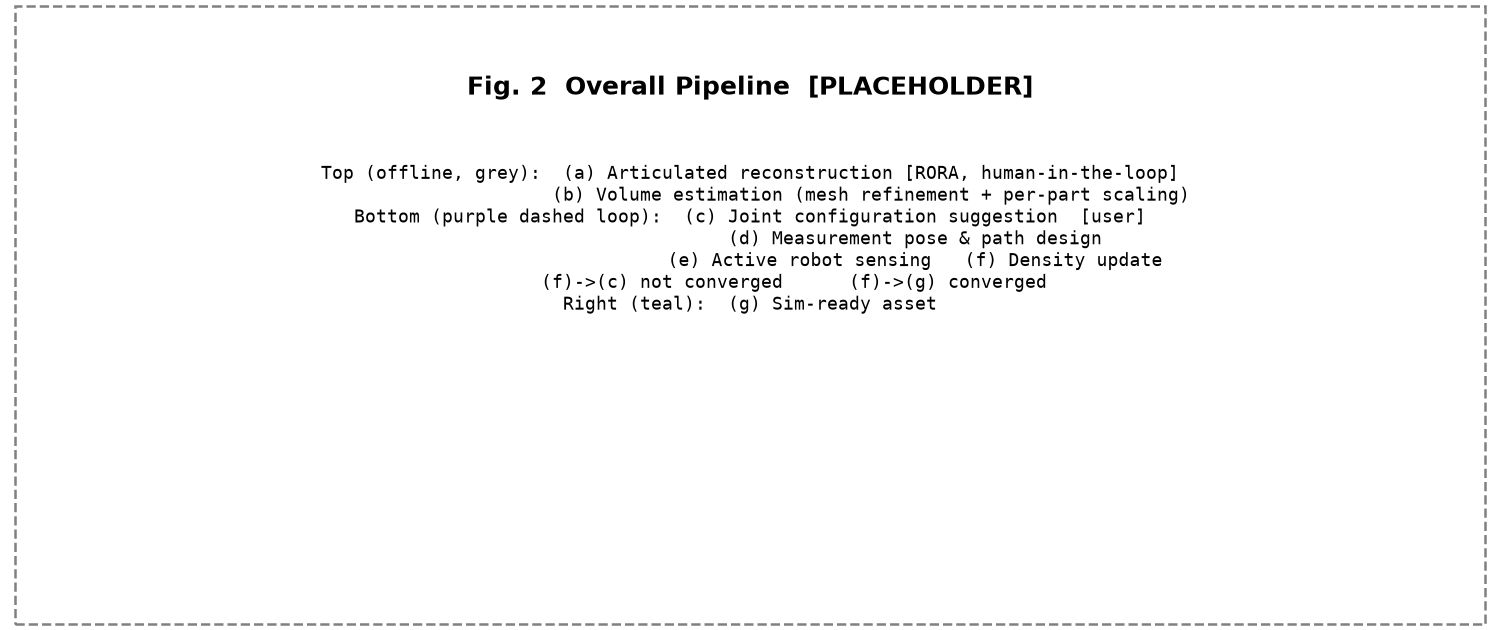
\includegraphics[width=\textwidth]{fig2_pipeline.png}
\caption{Pipeline. From the asset of~\cite{lee2026rora}, the offline
stage estimates part volumes; the closed loop suggests joint configurations,
reorients the object to three gravity directions, and updates part densities
until convergence.}
% [번역] 파이프라인. [RORA] 의 자산에서 오프라인 단계가 part 부피를
%   추정하고, 폐루프가 joint configuration 을 제안하며 물체를 중력 방향
%   3개로 재배치하고 수렴까지 part 밀도를 갱신한다.
%   ("추가 개입은 제시된 joint configuration 조정뿐" 은 초록·IV-E 산문에.)
\label{fig:pipeline}
\end{figure*}


RORA~\cite{lee2026rora} reconstructs the object from a video of one static
configuration: $P$ rigid parts, each with a mesh and 3D Gaussians, in a
metric-scale URDF. Part $i$ has volume $V_i$ and unknown uniform density
$\rho_i$; mass, center of mass, and inertia follow analytically, so
$\rho=(\rho_1,\dots,\rho_P)^{\!\top}$ alone separates a visually faithful
asset from a dynamically faithful one.
% [번역] RORA 는 단일 정적 형상을 담은 영상 하나에서 물체를 재구성한다.
%   mesh 와 3D Gaussian 을 가진 강체 part P 개가 계량 축척의 URDF 를 이룬다.
%   part i 는 부피 V_i 와 알려지지 않은 균일 밀도 rho_i 를 갖고 질량·
%   무게중심·관성은 해석적으로 따라 나오므로, rho 하나가 시각적으로 충실한
%   asset 과 동역학까지 충실한 asset 을 가른다.

A gripper rigidly grasps the object behind a wrist force/torque sensor
(frame $\mathcal{S}$); the configuration
$\theta\in\Theta\subset\mathbb{R}^{J}$ is friction-held, operator-set, and
camera-read---known only up to measurement error. The wrist is
quasi-statically reoriented through gravity directions $\hat g$, reading the
wrench $y=(f,\tau)$ after tare.
% [번역] 그리퍼가 손목 force/torque 센서(좌표계 S) 뒤에서 물체를 단단히
%   잡는다. 관절 형상 theta 는 마찰로 유지되고 작업자가 맞추며 RGB-D
%   카메라로 읽히므로 측정 오차만큼만 불확실하게 알려진다. 손목은 준정적으로
%   여러 중력 방향을 거치고, 타어링 뒤 렌치 y = (f, tau) 를 읽는다.

The wrench is linear in $\rho$: with
%
\begin{equation}
v \triangleq (V_1,\dots,V_P)^{\!\top}\!,\;\;
C(\theta) \triangleq
\big[\,V_1c_1(\theta)\;\cdots\;V_Pc_P(\theta)\,\big]
\in\mathbb{R}^{3\times P}\!,
\label{eq:vC}
\end{equation}
%
where $c_i(\theta)$ is the centroid of part $i$ in $\mathcal{S}$,
%
\begin{equation}
y \;=\; A(\theta,\hat g)\,\rho+\varepsilon,
\qquad
A(\theta,\hat g)=g\!\begin{bmatrix}\hat g\,v^{\!\top}\\[2pt]
-[\hat g]_\times C(\theta)\end{bmatrix}\!\in\mathbb{R}^{6\times P}.
\label{eq:regressor}
\end{equation}
%
$A$ needs volumes and centroids only---no density; noise is
$R=\mathrm{blkdiag}(\sigma_f^2I_3,\sigma_\tau^2I_3)$; one weighing of the
assembled object gives $v^{\!\top}\!\rho$, seeding the prior.
% [번역] 렌치는 rho 에 선형이다. 형상을 식 (1) 로 모으면 — c_i(theta) 는 S
%   에서 본 part i 의 도심 — 측정 모형 (2) 를 얻는다. A 는 부피와 도심만
%   쓰므로 밀도를 몰라도 계산된다. 잡음은 블록 등방이고, 조립된 물체를 한 번
%   저울에 올리면 v^T rho 가 나와 사전분포를 초기화한다.

The estimation vector must count every mass the wrench feels: small, occluded
hardware---above all the friction hinges holding $\theta$, $41\,\mathrm{g}$
in $7.45\,\mathrm{cm}^3$ on our custom objects---enters $\rho$ as its own
component. Omitted, the hinge mass biases by $79.1\%$ while the reported
half-width stays $0.83\%$---confidently wrong, unrepaired by more rounds.
% [번역] 추정 벡터는 렌치가 느끼는 모든 질량을 세어야 한다. 작고 가려진
%   하드웨어 — 무엇보다 theta 를 붙잡는 마찰 힌지, 커스텀 물체에서 7.45
%   cm^3 에 41 g — 는 rho 의 독립 성분으로 들어간다. 빼면 힌지 질량이
%   79.1 % 편향되면서도 보고되는 반폭은 0.83 % 에 머문다 — 라운드를 더해도
%   고쳐지지 않는, 틀렸는데 맞았다고 확신하는 답이다.

PIVoT closes a loop around this model (Fig.~\ref{fig:pipeline}): an offline
stage (Sec.~\ref{sec:geom}) produces the volumes and centroids behind every
regressor; each round selects the most informative joint
configuration---set by hand by the operator, the only intervention added
beyond those inherited from reconstruction---then measures along designed
poses and paths and updates the posterior over $\rho$ until a target
relative uncertainty is met.
% [번역] PIVoT 는 이 모형 둘레로 폐루프를 돈다. 오프라인 단계(III-B)가 모든
%   회귀행렬의 재료인 부피와 도심을 만들고, 각 라운드는 가장 정보량 높은
%   관절 형상을 골라 — 작업자가 손으로 맞추며, 재구성 단계에서 상속되는 개입
%   외에 추가되는 유일한 개입이다 — 설계된 자세·경로를 따라 렌치를 재어
%   rho 의 사후분포를 갱신하고, 목표 상대 불확실도에 닿을 때까지 돈다.

\subsection{Part-Wise Volume Estimation}
\label{sec:geom}

This stage turns the captured views and RORA's meshes into the $V_i$ and
$c_i(\theta)$ of \eqref{eq:vC}: mesh refinement enforces multi-view
consistency \rev{[pending: refinement implementation from collaborator]},
then each part is rescaled along its principal (PCA) axes against the
anisotropic scale error that survives
\rev{[pending: refinement implementation from collaborator]}. Volumes and
centroids are integrated from the result (non-watertight meshes via their
exactly integrable convex-decomposition union); CAD solids
and direct measurement serve as ground truth, never pipeline inputs.
% [번역] 이 단계는 촬영 시점들과 RORA 의 mesh 를 식 (1) 의 V_i 와 도심으로
%   바꾼다. mesh refinement 가 multi-view consistency 를 강제하고 [협업자
%   구현 대기], 이어 각 part 를 주축(PCA) 방향으로 재배율해 남는 비등방 배율
%   오차를 보정한다 [협업자 구현 대기]. 부피와 도심은 그 결과에서 적분하되
%   수밀하지 않은 mesh 는 볼록 분해의 합집합(적분이 정확함)으로 대체한다.
%   CAD 솔리드와 직접 측정은 채점 기준이지 파이프라인 입력이 아니다.

\begin{remark}[Volume invariance]
\label{rem:volume}
In \eqref{eq:vC}--\eqref{eq:regressor} the measurement depends on $\rho$ only
through the products $V_i\rho_i$: for fixed centroids, replacing each $V_i$ by
any $V'_i>0$ and $\rho_i$ by $(V_i/V'_i)\rho_i$ leaves $A(\theta,\hat g)\rho$
unchanged. The estimated part masses $\hat m_i=V_i\hat\rho_i$ are therefore
invariant to volume error, which enters only the derived density
$\hat\rho_i=\hat m_i/V_i$.
\end{remark}
% [번역] 비고 (부피 불변성). 식 (1)-(2) 에서 측정은 rho 에 오직 곱 V_i rho_i
%   를 통해서만 의존한다. 도심을 고정한 채 V_i 를 V'_i 로 바꾸고 rho_i 를
%   (V_i/V'_i) rho_i 로 두면 A rho 가 그대로다. 따라서 추정 part 질량은 부피
%   오차에 불변이고, 부피 오차는 파생 밀도에만 들어온다.

The invariance is exactly that narrow---its limits are what ``volume-aware''
means: density inherits volume error one-to-one
($\hat\rho_i=\hat m_i/V_i$), inertia keeps $s^2$ of a scale error $s$, and
centroids enter $C(\theta)$ itself, corrupting the estimated \emph{masses}
by ${\sim}2.4\%$ per millimetre. Were part masses the goal, refinement would
be needless by Remark~\ref{rem:volume}; a sim-ready asset also needs
density, inertia, and centroids (verified in Sec.~\ref{sec:vol}).
% [번역] 이 불변성은 딱 그만큼만 성립하며, 그 한계가 "volume-aware" 가
%   뜻하는 바다. 밀도는 부피 오차를 1:1 로 물려받고, 관성은 배율 오차 s 의
%   s^2 배가 남으며, 도심은 C(theta) 에 들어가 추정 '질량' 을 mm 당 약
%   2.4 % 오염시킨다. 목표가 part 질량뿐이면 Remark 1 에 의해 정제가
%   불필요하지만 sim-ready asset 은 밀도·관성·도심까지 맞아야 한다
%   (수치 확인은 IV-B).

\subsection{Information-Theoretic Joint Configuration Selection}
\label{sec:theory}\label{sec:design}

The classical limit of static gravity
sensing~\cite{atkeson1986estimation} becomes, in density coordinates:
% [번역] 밀도 좌표에서, 정지 중력 측정의 고전적 한계는 다음 형태가 된다.

\begin{lemma}[Closed-form information; classical fact restated]
\label{lem:closed}
For any finite set $\mathcal{G}=\{\hat g_k\}_{k=1}^{K}$ of unit gravity
directions, the Fisher information about $\rho$ gathered at configuration
$\theta$ is
\begin{equation}
M(\theta;\mathcal{G})=g^2\!\left[\frac{K}{\sigma_f^2}vv^{\!\top}
+\frac{1}{\sigma_\tau^2}C^{\!\top}\!\Big(KI_3-\!\sum_k\hat g_k\hat g_k^{\!\top}
\Big)C\right].
\label{eq:closed}
\end{equation}
\end{lemma}
% [번역] 보조정리 1 (닫힌 형태의 정보행렬; 고전적 사실의 재진술). 단위 중력
%   방향의 임의의 유한 집합 G 에 대해, 형상 theta 에서 rho 에 관해 모이는
%   Fisher 정보는 위 식과 같다.

\begin{IEEEproof}
Expand $A^{\!\top}R^{-1}A$ using
$[\hat g]_\times^{\!\top}[\hat g]_\times=I_3-\hat g\hat g^{\!\top}$; sum over
$k$.
\end{IEEEproof}
% [번역] 증명. A^T R^-1 A 를 [g_hat]_x^T [g_hat]_x = I_3 - g_hat g_hat^T 로
%   전개하고 k 에 대해 더한다.

\begin{corollary}[Triad invariance]
\label{cor:invariance}
If $\mathcal{G}$ is an orthonormal basis then $\sum_k\hat g_k\hat g_k^{\!\top}
=I_3$ and
\begin{equation}
M(\theta)=g^2\!\left[\tfrac{3}{\sigma_f^2}vv^{\!\top}
+\tfrac{2}{\sigma_\tau^2}C(\theta)^{\!\top}C(\theta)\right],
\label{eq:triad}
\end{equation}
which is invariant to rotating the whole triad by any $Q\in SO(3)$.
\end{corollary}
% [번역] 따름정리 1 (삼면체 불변성). G 가 직교정규 기저이면 정보행렬이 위
%   형태로 줄고, 삼면체 전체를 임의의 Q in SO(3) 로 돌려도 변하지 않는다.

Cor.~\ref{cor:invariance} collapses the design space to $\Theta$: wrist tilt
carries no information, so articulation is the \emph{only} design variable;
the freed $SO(3)$ is spent in Sec.~\ref{sec:path}. And since $M(\theta)$ is
independent of $\rho$, the loop exists only to absorb angle error.
% [번역] 따름정리 1은 설계 공간을 Theta 로 접는다. 손목 기울임은 정보를
%   나르지 않으므로 관절 형상이 유일한 설계 변수이고, 풀려난 SO(3) 는 III-D
%   에서 조작 실현 가능성에 쓰인다. M(theta) 는 rho 와도 무관하므로,
%   폐루프는 오직 각도 오차를 흡수하기 위해 존재한다.

\begin{proposition}[Rank ceiling]
\label{prop:rank}
For any $K$ and any arrangement of gravity directions,
$\operatorname{rank}M(\theta;\mathcal{G})\le1+\operatorname{rank}C(\theta)
\le1+\min(3,P)$.
\end{proposition}
% [번역] 명제 1 (rank 천장). 중력 방향의 개수와 배치가 어떠하든
%   rank M <= 1 + rank C(theta) <= 1 + min(3, P) 이다.

Its proof---PSD ordering plus rank subadditivity---is standard.
% [번역] 식 (3) 의 두 항은 준양정이고(g g^T <= I_3), rank 준가법성이 표준
%   증명을 끝낸다.

\begin{corollary}[Rigid objects are capped at four]
\label{cor:rigid}
Holding the configuration fixed, no number of gravity directions or repeated
measurements raises the rank above four: a rigid assembly of $P\ge5$ parts is
not identifiable from quasi-static wrench sensing without additional
priors---the closure rigid-object
methods~\cite{nadeau2023sum,pfaff2025scalable,shuai2025pugs} must buy.
\end{corollary}
% [번역] 따름정리 2 (강체는 넷에서 막힌다). 형상을 고정하면 중력 방향과 측정
%   반복을 몇 번 쓰든 rank 가 4 를 넘지 않는다. P >= 5 인 강체 조립품은
%   추가 사전지식 없이 정지 렌치 측정만으로 식별할 수 없다.

\begin{proposition}[What stays invisible]
\label{prop:null}
With an orthonormal triad,
$\mathcal{N}(M(\theta))=\{u:\sum_iu_iV_i=0\ \text{and}\ \sum_iu_iV_ic_i(\theta)
=0\}$: a redistribution of mass preserving both the total mass and the first
moment about the sensor origin is unobservable at $\theta$.
\end{proposition}
% [번역] 명제 2 (무엇이 끝내 보이지 않는가). 직교정규 삼면체에서 M(theta) 의
%   영공간은 총질량과 센서 원점 기준 1차 모멘트를 둘 다 보존하는 재분배 u
%   전체와 같다. 그런 재분배는 theta 에서 관측되지 않는다.

\begin{IEEEproof}
With $M=a\,vv^{\!\top}+b\,C^{\!\top}C$, $a,b>0$:
$Mu=0\iff a(v^{\!\top}u)^2+b\|Cu\|^2=0\iff v^{\!\top}u=0$, $C(\theta)u=0$.
\end{IEEEproof}
% [번역] 증명. M = a vv^T + b C^T C (a, b > 0) 로 쓰면 Mu = 0 은
%   a(v^T u)^2 + b||Cu||^2 = 0, 곧 v^T u = 0 이면서 C(theta) u = 0 과
%   동치다.

A redistribution hidden at $\theta_1$ becomes visible at $\theta_2$ iff
$C(\theta_2)u\neq0$; only articulation moves $C$---the method is specific to
articulated objects, not merely applicable: a redistribution of
$+100/-200/+100\,\mathrm{g}$ preserving total mass and first moment is
invisible at every wrist orientation, and folding the joint moves the far
centroid and reveals it.
% [번역] theta_1 에서 숨은 재분배가 theta_2 에서 보이는 것은 정확히
%   C(theta_2) u != 0 일 때이고, C 를 움직이는 유일한 수단이 관절 운동이다.
%   이 방법은 관절 물체에 '적용 가능한' 정도가 아니라 고유하다. 예를 들어
%   +100/-200/+100 g 의 재분배는 총질량과 1차 모멘트를 보존하므로 손목을 어떻게
%   돌려도 보이지 않고, 관절을 접으면 먼 쪽 도심이 움직여 드러난다.
%   [8/30] 가이드라인 v2 의 [Figures] 목록에 없는 그림이라 영공간 도식을 삭제하고
%   그 내용을 이 문장에 흡수했다. 그림 파일은 figures/fig_nullspace.pdf 에 남아 있다.


\begin{proposition}[Lower bound on rounds]
\label{prop:rounds}
With $M_R=\sum_{r=1}^{R}M(\theta_r)$ we have
$\operatorname{rank}M_R\le1+\min(3R,P)$, so identifying all $P$ densities
requires $R\ge\lceil(P-1)/3\rceil$ distinct configurations.
\end{proposition}
% [번역] 명제 3 (라운드 하한). R 개 형상의 정보를 합한 M_R 은 rank M_R <=
%   1 + min(3R, P) 이므로, 밀도 P 개를 전부 식별하려면 서로 다른 형상이
%   R >= ceil((P-1)/3) 개 필요하다.

The proof stacks the $C(\theta_r)$ and applies subadditivity to the Gram
matrix. For a serial chain of $p$ links with a friction hinge
per joint, $P=2p-1$:
\begin{equation}
R\;\ge\;\big\lceil (2p-2)/3\big\rceil ,
\label{eq:chain}
\end{equation}
met with equality on both custom objects (Sec.~\ref{sec:pred}). In density
coordinates, the geometric observability characterization
of~\cite{wensing2024geometric}, specialized to quasi-static gravity, is
exactly Props.~\ref{prop:rank} and~\ref{prop:null}; the configuration count
of Prop.~\ref{prop:rounds} is what the density view adds.
% [번역] 증명은 C(theta_r) 을 3R x P 행렬로 쌓아 그 그람 행렬에 rank
%   준가법성을 적용하면 끝난다. p 개 링크가 직렬이고 관절마다 마찰 힌지가
%   달린 사슬에서는 P = 2p-1 이라 식 (5) 로 특수화되며, 커스텀 물체 둘 모두
%   등호로 만족한다(IV-C). Wensing 등의 기하학적 관측가능성 특성화를 중력만의
%   준정적 측정으로 특수화하면 밀도 좌표에서 정확히 명제 1·2가 된다. 형상이
%   몇 개 필요한가를 세는 명제 3이 밀도 관점이 더하는 것이다.

\begin{remark}[Channel separation]
\label{rem:channel}
The force block $-g(v^{\!\top}\!\rho)\hat g$ of \eqref{eq:regressor} is
free of $\theta$: joint-angle error enters
$R_{\mathrm{eff}}=R+J\Sigma_\theta J^{\!\top}$ through the torque rows alone.
Rank one with row space $\mathrm{span}\{v\}$, it determines only the total
mass the scale provides; the part-separating and angle-corrupted subspaces
coincide, so reducing $\sigma_f$ improves nothing the scale has not fixed.
\end{remark}
% [번역] 비고 (채널 분리). 힘 블록 -g (v^T rho) g_hat 에는 theta 가 없으므로
%   관절각 오차는 R_eff 에 오직 토크 행으로만 들어온다. 같은 블록은 rank 1,
%   행공간 span{v} 라 저울이 이미 주는 총질량만 결정한다. 부위를 가르는
%   부분공간과 각도 오차가 오염시키는 부분공간이 일치하므로, sigma_f 를
%   줄여도 저울이 이미 고정한 것 밖은 개선되지 않는다.

\begin{remark}[Necessary, not sufficient]
\label{rem:cond}
Prop.~\ref{prop:rounds} constrains rank only and grows \emph{additively}:
two unknowns per link buy at most a third of a round. Once $M_R$ is full
rank, conditioning governs, degrading \emph{multiplicatively}---roughly
twofold per link, hence with half-width $\propto1/\sqrt{R}$ roughly fourfold
more rounds per link (quantified in Sec.~\ref{sec:sim}).
\end{remark}
% [번역] 비고 (필요조건이지 충분조건이 아니다). 명제 3은 rank 만 구속하며
%   '덧셈' 으로 는다(링크당 미지수 둘, 라운드는 많아야 1/3). M_R 이 full
%   rank 가 된 뒤에는 조건수가 지배하고 이는 '곱셈' 으로 나빠진다 — 우리
%   사슬에서 링크당 약 2배, 반폭이 1/sqrt(R) 이므로 라운드는 약 4배
%   (정량화는 IV-C).

Each round maximizes expected information gain under the current posterior
$\Sigma$,
%
\begin{equation}
\theta^\star=\arg\max_{\theta\in\Theta_{\mathrm{feas}}}\;
\tfrac{1}{2}\log\det\!\big(I+R_{\mathrm{eff}}^{-1/2}A(\theta)\Sigma
A(\theta)^{\!\top}\!R_{\mathrm{eff}}^{-1/2}\big),
\label{eq:dopt}
\end{equation}
%
on the relative-uncertainty scaling of $\Sigma$. The triad drops out
(Cor.~\ref{cor:invariance}): the search runs over joint angles only, by
multi-start optimization over $\Theta_{\mathrm{feas}}$ of
Sec.~\ref{sec:path}. \eqref{eq:dopt} is classical
D-optimality~\cite{gautier1992exciting,swevers1997optimal};
ours differs in procedure, not criterion: the design variable is the
object's own articulation, not the robot's trajectory, and $\Sigma$ is the
per-round posterior, not a prior optimized once.
% [번역] 매 라운드는 현재 사후분포 Sigma 아래 기대 정보이득을 최대화하며
%   (식 6), Sigma 의 상대 불확실도 스케일 위에서 평가한다. 따름정리 1로
%   삼면체가 사라지므로 탐색은 관절각에 대해서만, III-D 의 실현 가능 집합
%   Theta_feas 위에서 다중 출발 연속 최적화로 푼다. 식 (6) 은 고전적 D-최적
%   기준이다. 우리가 다른 것은 기준이 아니라 절차다. 설계 변수가 로봇 궤적이
%   아니라 물체 자신의 관절 형상이고, Sigma 는 1회 최적화된 사전분포가 아니라
%   매 라운드 갱신되는 사후분포다.

The accepted $\theta^\star$ goes to the operator: the robot holds still, the
interface shows the target angles, and the operator sets the joints by
hand---the one intervention PIVoT adds beyond reconstruction; the robot
proceeds only after the camera reads the achieved angles.
% [번역] 채택된 theta* 는 작업자에게 간다. 로봇은 정지하고 인터페이스가 목표
%   관절각을 표시하며 작업자가 관절을 손으로 맞춘다 — PIVoT 가 재구성 너머로
%   추가하는 유일한 개입이다. 로봇은 카메라가 실제 각도를 읽은 뒤에만
%   움직인다.

\subsection{Multi-Topology Measurement Path Design}
\label{sec:path}

Each configuration is measured at three poses forming an orthonormal gravity
triad---not for observability: two non-parallel directions already attain the
rank ceiling of Prop.~\ref{prop:rank} (for $K=2$ the weighting in
\eqref{eq:closed} is positive definite). The third direction completes
$\sum_k\hat g_k\hat g_k^{\!\top}=I_3$ (Cor.~\ref{cor:invariance}):
information becomes isotropic, the ceiling is met at the direction set's best
conditioning, and the triad's $SO(3)$ orientation becomes informationally
\emph{free}. Measurement agrees (Sec.~\ref{sec:posepath}).
% [번역] 형상마다 직교정규 중력 삼면체를 이루는 측정 자세 3개에서 재는데,
%   이유는 관측가능성이 아니다. 비평행 2방향이면 이미 명제 1의 rank 천장에
%   도달한다(K=2 에서 식 (3) 의 가중이 양정). 세 번째 방향은 sum g g^T =
%   I_3 을 완성해(따름정리 1) 정보를 등방으로 만들고, 방향 집합이 줄 수 있는
%   최선의 조건수에서 천장을 달성하며, 삼면체의 SO(3) 방향을 정보 면에서
%   '공짜' 로 만든다. 실측이 이를 뒷받침한다(IV-D).

The free orientation pays for manipulation: rotating the whole triad changes
nothing in \eqref{eq:triad}, so we rotate it for grasp feasibility,
reachability, collision avoidance, and joint protection at zero informational
cost (quantified in Sec.~\ref{sec:posepath}).
% [번역] 공짜인 방향이 조작의 값을 치른다. 삼면체를 통째로 돌려도 식 (4) 는
%   변하지 않으므로, 정보 비용 0 으로 파지 가능성·도달성·충돌 회피·관절
%   보호를 만족하도록 돌린다(정량화는 IV-D).

Because $\theta$ changes the object's \emph{shape}, feasibility is re-checked
per candidate---identification design under restricted
trajectories, with a shape-changing payload:
$\theta^\star$ must admit grasping and holding at all three poses without
collision, across the tracker's angular-uncertainty interval, plus a
collision-free inter-pose path \emph{under the shape at that configuration}
(planning against the previous round's shape collides in transit). Failing
candidates are excluded with a neighbourhood; \eqref{eq:dopt} is re-solved.
% [번역] theta 가 물체의 '모양' 을 바꾸므로 후보마다 실현 가능성을 다시
%   따진다 — 실현 가능한 궤적이 제한된 식별 설계의, 페이로드가 모양을 바꾸는
%   판본이다. theta* 는 세 자세 모두에서 충돌 없이 잡고 유지할 수 있어야
%   하고, 추적기의 각도 불확실 구간 전체에서 그래야 하며, 자세 간 충돌 없는
%   경로가 '그 형상의 모양 아래' 존재해야 한다(직전 라운드의 모양으로
%   계획하면 이동 중 충돌한다). 실패 후보는 근방과 함께 배제하고 식 (6) 을
%   다시 푼다.

Paths are planned by RRT-Connect in the arm's joint space with the object
rigidly attached, checking joint limits, environment and self-collisions,
and the object's own collision pairs. Topology changes the problem, not its
parameters---spatial extent, active self-collision pairs, reachable
reorientations---so triad rotation and paths are re-solved per topology and
configuration. Joint visibility, too: an axis near the camera's line of
sight projects poorly (worst \rev{$0.37\,\mathrm{px/deg}$}, a
\rev{$4.1\times$} spread), so each joint is read where its axis is best
conditioned.
% [번역] 경로는 물체를 강체로 부착한 채 팔의 관절공간에서 RRT-Connect 로
%   계획하며 관절 한계, 환경·자기충돌, 물체 자신의 충돌 쌍을 검사한다.
%   topology 는 매개변수가 아니라 문제 자체를 바꾼다 — 공간 점유, 활성화될
%   자기충돌 쌍, 도달 가능한 재배치 — 그래서 삼면체 회전과 경로는 topology
%   마다, 형상마다 다시 푼다. 관절 가시성도 같은 설계에 든다. 카메라 시선과
%   거의 나란한 축은 투영이 나빠(최악 0.37 px/deg, 관절 간 4.1배 차이) 각
%   관절을 그 축이 가장 잘 조건화된 자세에서 읽는다.

\subsection{Active Sensing and Uncertainty-Aware Density Update}
\label{sec:estimation}

The robot keeps inertial forces below one percent of gravity, holds still at
each pose, and reads the wrench after tare. The regressed configuration is
the camera-\emph{measured} $\hat\theta$, so $A(\hat\theta)$ is corrupted:
errors-in-variables, under which weighted least squares stays biased however
many rounds accumulate.
% [번역] 로봇은 관성력을 중력의 1 % 아래로 유지하며 자세마다 정지해 타어링
%   뒤 렌치를 읽는다. 회귀에 쓰는 형상은 카메라가 '측정한' theta-hat 이므로
%   A(theta-hat) 자체가 오염되어 있다. 이 오차변수(EIV) 구조에서
%   가중최소제곱은 라운드를 아무리 쌓아도 편향된 채로 남는다.

We therefore estimate the per-round angle correction $\delta_r$ jointly with
$\rho$:
%
\begin{equation}
\min_{\rho,\{\delta_r\}}\;\sum_r\big\|y_r-A(\hat\theta_r+\delta_r)\rho\big\|^2
_{R_{\mathrm{eff}}^{-1}}
+\sum_r\|\delta_r\|^2_{\Sigma_\theta^{-1}}
+\|\rho-\mu_0\|^2_{\Sigma_0^{-1}},
\label{eq:tls}
\end{equation}
%
under positivity box constraints,
with $\Sigma_\theta$ the tracker's angle covariance and the prior seeded by
the scale---the total-least-squares remedy
applied to the design variable itself. A grasp offset $\delta$ adds
$MG[\hat g]_\times\delta$ to the torque rows---three linear unknowns, $M$
known from the scale. The posterior propagates
with $R_{\mathrm{eff}}=R+J\Sigma_\theta J^{\!\top}$,
$J=\partial(A\rho)/\partial\theta$.
% [번역] 그래서 라운드별 각도 보정 delta_r 을 rho 와 함께 추정한다(식 7).
%   모든 밀도를 양수로 유지하는 상자 제약 아래 풀고, Sigma_theta 는 추적기의
%   각도 공분산, 사전분포는 저울 값으로 초기화한다 — 총최소제곱 해법을 설계
%   변수 자신에 적용한 것이다. 파지 오프셋 delta 는 토크 행에 들어오는데
%   총질량 M 을 저울에서 알므로 선형 미지수 셋만 더한다. 사후분포는 R_eff =
%   R + J Sigma_theta J^T 로 순차 전파한다.

Because \eqref{eq:tls} fits $y\approx A(\hat\theta+\delta)\rho$, residuals
must be scored at $\hat\theta_r+\delta_r$: scoring at $\hat\theta$ charges
the recovered correction back to the residual---interval inflation of
\rev{$79\times$} at $p=4$, the stopping test never satisfied though the
estimate is accurate to \rev{$0.28\%$}---a structural trap of pairing an
errors-in-variables estimator with a residual-based stopping rule.
% [번역] 식 (7) 은 y ≈ A(theta-hat + delta) rho 를 맞추므로 잔차도 보정된
%   형상에서 채점해야 한다. theta-hat 에서 채점하면 방금 복원한 보정이
%   잔차로 청구되어 구간 팽창이 p=4 에서 79배에 이르고, 추정이 이미 0.28 %
%   로 정확한데도 정지 조건이 끝내 만족되지 않는다. 오차변수 추정기를 잔차
%   기반 정지 규칙과 짝지을 때의 구조적 함정이다.

The loop stops when the $95\%$ relative half-width over the \emph{parts}
falls below $\tau(p)=0.5\%\times p$ ($1.0$--$3.0\%$ for $p=2$--$6$), inflated
when the residual exceeds the noise prediction; the per-part budget follows
from Remark~\ref{rem:cond}. Hinge rows known from the scale are excluded lest
their prior width block termination, and the iteration budget scales with
$P+RJ$. Unmet, $\Sigma$ re-enters \eqref{eq:dopt}.
% [번역] 루프는 'part' 에 대한 95 % 상대 반폭이 링크 수 비례 목표 tau(p) =
%   0.5 % x p (p = 2..6 에서 1.0~3.0 %) 아래로 내려가면 멈추고, 잔차가 잡음
%   예측을 넘으면 반폭을 부풀린다. 부위당 예산은 비고 3에서 나온다. 저울에서
%   이미 아는 힌지 행은 사전 폭이 종료를 막지 못하도록 제외하고, 반복 예산은
%   미지수 개수 P + RJ 에 따라 늘린다. 목표에 못 미치면 Sigma 가 식 (6) 에
%   다시 들어간다.

One quantity is beyond this loop by physics, not design: the inertia tensor
cannot be identified quasi-statically---at rest $\omega=0$ and $\alpha=0$, so
every term of $\tau=I\alpha+\omega\times(I\omega)$ containing $I$ vanishes
identically, and the static wrench constrains only the zeroth and first mass
moments (Prop.~\ref{prop:rank}). Exported inertia is \emph{derived}---mesh
geometry times identified density under the uniform-density assumption---not
measured, inheriting volume-scale error as $s^2$ (Sec.~\ref{sec:geom}) and
bounding what any quasi-static method can claim.
% [번역] 한 가지 양은 설계가 아니라 물리에 의해 이 루프 바깥에 있다. 회전
%   관성 텐서는 준정적으로는 식별할 수 없다. 정지 상태에서 omega = 0,
%   alpha = 0 이므로 tau = I alpha + omega x (I omega) 에서 I 를 담은 모든
%   항이 항등적으로 사라지고, 정지 렌치는 0차·1차 질량 모멘트만 구속한다
%   (명제 1). 따라서 내보내는 관성은 측정값이 아니라 '유도값' — 균일 밀도
%   가정 아래 mesh 기하 곱하기 식별된 밀도 — 이며 부피 배율 오차를 s^2 로
%   물려받는다(III-B). 준정적 방법이 주장할 수 있는 것의 경계다.

The converged $\hat\rho$ yields each part's mass, center of mass, and derived
inertia analytically, written into the URDF with geometry, joints, and
Gaussians untouched; the asset is revalidated in simulation at measured
and held-out configurations.
% [번역] 수렴한 rho-hat 에서 각 part 의 질량·무게중심·유도 관성이
%   해석적으로 나와 URDF 에 기록되며, 형상·관절·Gaussian 은 건드리지
%   않는다. asset 은 시뮬레이션에서 측정 형상과 보지 않은 형상 모두로
%   재검증한다.

%%%%%%%%%%%%%%%%%%%%%%%%%%%%%%%%%%%%%%%%%%%%%%%%%%%%%%%%%%%%%%%%
% [메모] 8/30 압축판 (COMPRESSION_RULES.md, 목표 1,500 단어).  구조는 v2
%   5소절 그대로: A Setup / B Volume / C Density (main) / D Pose & Path /
%   E Asset.  수치 출처 불변: RESULTS.md (E1~E10), gt.json, frozen vision 열,
%   figures/v2/*.json.  없는 값은 \Pending / \rev.  실물 로봇 데이터 없음.
%   Exp E 는 시뮬-시뮬 대리 검증으로만 서술.  라벨 호환: sec:vol / sec:sim /
%   sec:pred 유지.  Table I 은 실제 표로 복원 (tables/table1_objects_v2.tex,
%   tab:objects 라벨은 표 안).  실물 비교 자리표시자 그림(구 Fig. 8)은 Fig. 7
%   캡션에 흡수 (fig:assetreal 라벨은 그림 안에 보존).  표 캡션·각주가 이미
%   말하는 문장은 산문에서 지웠고, 잘린 산문은 CUTS.md 에 보관.

\section{Experiments}
\label{sec:exp}

\subsection{Setup}
\label{sec:setup}

\begin{figure}[!htb]
\centering
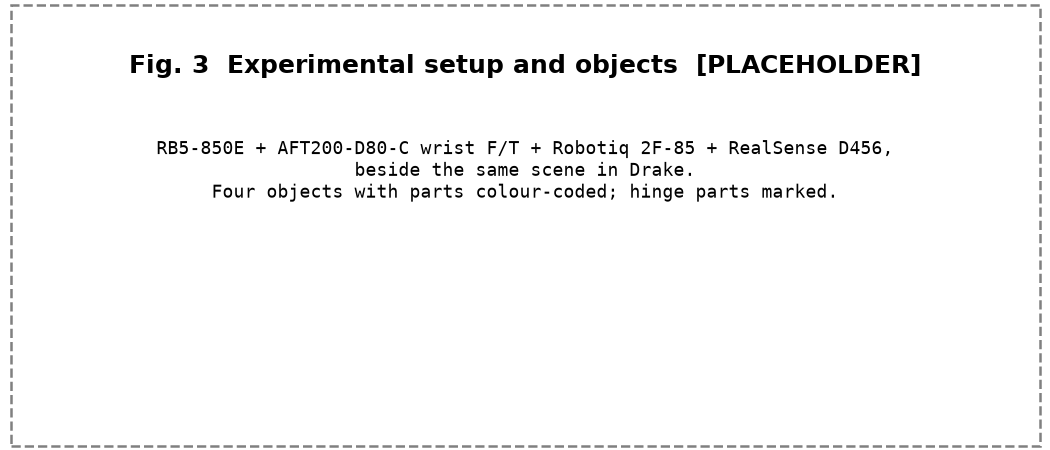
\includegraphics[width=\linewidth]{fig3_setup.png}
\caption{Experimental platform and the four evaluation objects of
Table~\ref{tab:objects}. \rev{[Placeholder: the photo awaits the hardware
session.]}}
% [번역] 그림 3 — 실험 플랫폼과 평가 물체 4종(표 I). 실물 사진은 하드웨어
%   세션 대기 자리표시자. 물체 사양(링크/P/rank/R_min/참값 출처)과 힌지
%   각주는 표 I 로 복원.
\label{fig:setup}
\end{figure}

% Table 1 — 실험 물체 사양.  출처: gt.json (gt_list.md 를 정본으로 재계산),
%   rank / R_min 은 my_work/study_theory.py 의 수치 검증 결과.
\begin{table}[t]
\caption{Evaluation objects: links, independently unknown densities $P$,
single-configuration rank $1+\min(3,P)$ (Prop.~\ref{prop:rank}), configuration
lower bound $R_{\min}=\lceil (P-1)/3\rceil$ (Prop.~\ref{prop:rounds}), and
ground-truth source.}
% [번역] 평가 물체: 링크 수, 독립 미지 밀도 P, 단일 형상 rank 1+min(3,P)
%   (명제 1), 형상 개수 하한 R_min = ceil((P-1)/3) (명제 3), 참값 출처.
\label{tab:objects}
\centering
\footnotesize
\setlength{\tabcolsep}{4pt}
\begin{tabular}{lccccl}
\toprule
Object & Links & $P$ & rank & $R_{\min}$ & Ground truth \\
\midrule
Custom 2-link  & 2 & 3$^{\mathrm h}$ & 3 & 1 & CAD $+$ material \\
Custom 3-link  & 3 & 5$^{\mathrm h}$ & 4 & 2 & CAD $+$ material \\
Stand lamp     & 3 & 3 & 3 & 1 & scan $+$ disassembly \\
Laptop$^{\dagger}$ & 2 & 2 & 3 & 1 & scale $+$ part split \\
\bottomrule
\end{tabular}
\vspace{2pt}
\parbox{\linewidth}{\footnotesize \textit{Rank and $R_{\min}$ follow from
geometry alone, before any wrench is measured. $^{\mathrm h}$ includes the friction hinge
as its own unknown ($41\,\mathrm{g}$ each). The hinge occupies $7.4\,\mathrm{cm^3}$ at
$5.51\,\mathrm{g/cm^3}$---small, largely occluded, and mass-dense, the case that makes
part-wise identification hard rather than the case that makes it easy.
$^{\dagger}$ \rev{Laptop mesh and URDF are in preparation; it contributes ground truth
and vision-baseline rows only.}}}
\end{table}



The platform: a six-axis RB5-850E arm, wrist force/torque sensor, Robotiq
2F-85 gripper, and one RealSense D456; joint angles are tracked on the
RGB-D stream---measured, not commanded (Fig.~\ref{fig:setup}). All
results below are Drake simulation, running the estimator, selection rule,
and stopping test of Sec.~\ref{sec:estimation} unchanged; \rev{the hardware runs
are in preparation, and every real-robot quantity is marked pending}.
% [번역] 장비: 6축 RB5-850E + 손목 F/T 센서 + Robotiq 2F-85 + RealSense D456
%   한 대. 관절각은 RGB-D 추적기의 측정값(명령값 아님)이다(그림 3). 아래 모든
%   결과는 III-E 의 추정기·선택 규칙·정지 판정을 그대로 돌린 시뮬레이션
%   (Drake)이다. 하드웨어 실행은 준비 중, 실물 수치는 전부 pending.

We evaluate four articulated objects (Fig.~\ref{fig:setup},
Table~\ref{tab:objects}): two custom 3D
prints with per-part densities we set, a disassembly-weighed stand lamp from
a 3DGS scan, and a laptop; the custom objects give their friction hinge its
own part---the harder general case. Density
identification covers three of the four: \rev{the laptop's mesh and URDF
assets are in preparation, so it contributes ground-truth and
vision-baseline rows only}.
% [번역] 평가 물체 4종(그림 3): 부위별 밀도를 지정한 커스텀 3D 프린트 2종,
%   분해 계량 참값의 3DGS 스캔 스탠드 램프, 노트북. 커스텀 둘은 마찰 힌지를
%   독립 part 로 둔다 — 작고 가려지고 질량이 몰린, 더 어려운 일반 경우. 밀도
%   식별은 4종 중 3종: 노트북 mesh/URDF 는 준비 중이라 참값·vision baseline
%   행만 기여한다.

Metrics: per-part relative density error; $95\%$ half-width and its
coverage (a confident wrong answer is worse than an uncertain one); rounds
to the target half-width $\tau=0.5\%\times P$; asset trajectory RMSE. All
methods share the same fixed part volumes, so density error and mass error
are the same number (Table~\ref{tab:main} footnotes). Four objects admit no
statistical-significance claim, so tables show per-part rows, not pooled
means.
% [번역] 지표: 부위별 상대 밀도오차, 보고 95 % 반폭과 경험적 커버리지(자신
%   있게 틀린 답이 불확실한 답보다 나쁘다), 목표 반폭 tau = 0.5 % x P 까지의
%   라운드 수, asset 은 궤적 RMSE. 모두 같은 고정 부피로 채점되므로 밀도오차
%   = 질량오차(1.7e-16 불변성은 표 III 각주). 물체 4개로는 통계적 유의성을
%   주장할 수 없어 표는 평균 아닌 부위별 행을 드러낸다.

Baselines are PUGS~\cite{shuai2025pugs}, SiPhy~\cite{le2026siphy}, and
PhysX-Omni~\cite{cao2026physxomni} from vision, plus three ablations:
\emph{uniform} (one density per assembly~\cite{pfaff2025scalable}),
\emph{single} (one fixed configuration, unlimited reorientations and
repeats~\cite{nadeau2023sum}), and \emph{WLS} (our loop, ignoring the
regressor's own angle error, Eq.~\eqref{eq:tls}). Vision outputs lacking
per-part densities are converted in whichever direction favors the baseline
(Table~\ref{tab:main} footnotes).
% [번역] baseline: vision 셋(PUGS, SiPhy, PhysX-Omni)과 ablation 셋 —
%   uniform 은 조립체에 밀도 하나, single 은 형상 하나 고정 + 무제한
%   reorientation·반복, WLS 는 우리 루프에서 회귀행렬 자체의 각도 오차(식
%   (7))만 무시. part 별 밀도가 없는 vision 출력은 매번 해당 baseline 에
%   유리한 방향으로 변환한다(표 III 각주).


\subsection{Part-Wise Volume Estimation}
\label{sec:vol}

\begin{figure*}[!t]
\centering
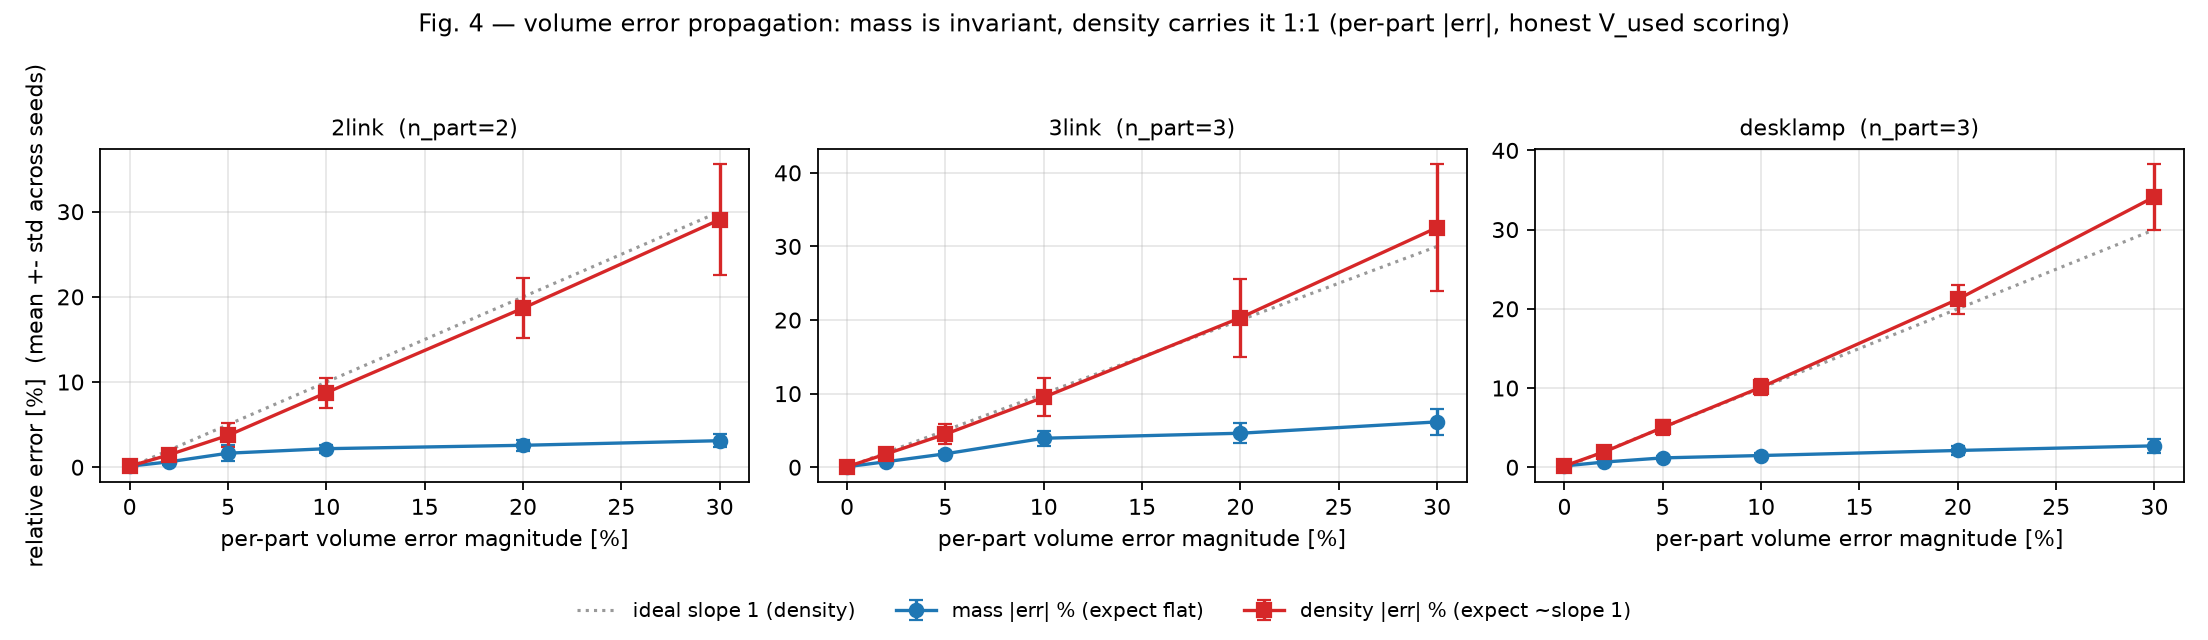
\includegraphics[width=0.74\textwidth]{fig_volume.png}
\caption{Injected part-volume error (eight seeds): density error tracks it
near one-to-one; part mass, scored with the volumes the estimator used,
drifts to $3$--$6\%$ at $\delta=30\%$---first-order invariant, not exactly
so.}
% [메모] Fig. 4 — 파일: figures/v2/fig_volume.png.
\label{fig:volume}
\end{figure*}


The CAD solids and displacement measurements are scoring references, never
inputs. \rev{The mesh refinement and per-part
scaling implementation is being delivered by a collaborator, so the measured
per-part volume-error table is deferred; no claim below depends on it.} What we can
already quantify is the downstream cost: we perturb the
volumes the estimator \emph{believes} by $\pm\delta$ with random signs while
measurements come from the true plant, scoring masses with the volumes
actually used ($\delta\le30\%$; Fig.~\ref{fig:volume}).
% [번역] CAD 솔리드·수중 배제 실측은 채점 기준이지 입력이 아니다.
%   refinement/scaling 구현은 협업자 인계 중이라 부피오차 실측 표는 유보,
%   아래 주장은 그에 의존하지 않는다. 지금 정량화할 수 있는 것은 하류 비용이다.
%   추정기가 '믿는' 부피를 ±delta 무작위 부호로 흔들되 측정은 참 plant 에서
%   나오고 질량은 실제 쓴 부피로 채점한다(delta <= 30 %, 그림 4).

Density error follows volume error near-exactly one-to-one; part mass is far
less sensitive but not exactly invariant---$3$--$6\%$ at $\delta=30\%$, the
MAP prior's cancellation being inexact (Remark~\ref{rem:volume} covers only
the least-squares core)---and the mesh-derived inertia tensor degrades as
$s^2$ ($19.1\%$ at $\delta=30\%$).
% [번역] 밀도오차는 부피오차를 거의 1:1 로 따르고, 부위 질량은 훨씬 덜
%   민감하나 엄밀히 불변은 아니며 — MAP 사전분포의 상쇄가 부정확해 delta
%   30 % 에서 3~6 % (Remark 의 불변성은 최소제곱 핵심만 다룬다) — mesh 유도
%   관성 텐서는 s^2 로 나빠진다(delta 30 % 에서 19.1 %).

Volume error also costs \emph{rounds}: the worst part drags the loop, median
rounds growing from $1$ to $7$ on the 2-link object by $\delta=30\%$, with
three of eight 3-link seeds failing to converge there. Refinement is what keeps the
interaction count bounded.
% [번역] 부피오차는 '라운드' 도 치른다. 최악 part 가 루프를 끌어 2링크에서
%   delta 30 % 까지 라운드 중앙값이 1 → 7 로 늘고, 3링크는 거기서 8 시드 중
%   3 이 미수렴. 상호작용 횟수를 유한하게 묶는 것이 바로 정제다.


% Table 2 (part별 부피 오차) 는 협업자의 refinement/scaling 실측이 도착할 때까지
% 전 칸이 Pending 이라 지면만 차지한다. 파일은 tables/table2_volume_v2.tex 에
% 그대로 두었으니, 자료가 오면 아래 한 줄의 주석만 풀면 된다.
% % Table 2 — part별 부피 오차.  refinement/scaling 구현과 실측 오차는 협업자 인계 대기.
%   빈 칸을 지어내지 않는다. 자료가 오면 \Pending 만 교체하면 된다.
\begin{table}[t]
\caption{Per-part volume error [\%] against the CAD solids (custom objects) and the
displacement measurements (stand lamp). The vision baselines are scored on the volume
they themselves recover---PUGS by integrating its Gaussians, PhysX-Omni on its generated
shape---so the table fixes how much of each method's density error is already present
before any density is assigned. \rev{The refinement and per-part scaling stage is being
delivered by a collaborator; its rows are pending.}}
\label{tab:volume}
\centering
\footnotesize
\setlength{\tabcolsep}{4pt}
\begin{tabular}{llccccc}
\toprule
& & \multicolumn{3}{c}{Baselines} & \multicolumn{2}{c}{Ours} \\
\cmidrule(lr){3-5}\cmidrule(lr){6-7}
Object & Part & Bbox & PUGS & \shortstack{PhysX-\\Omni} & \shortstack{raw\\mesh} & \shortstack{$+$refine\\$+$scale} \\
\midrule
\multirow{3}{*}{Stand lamp}
 & Base    & \Pending & \Pending & \Pending & \Pending & \Pending \\
 & Support & \Pending & \Pending & \Pending & \Pending & \Pending \\
 & Head    & \Pending & \Pending & \Pending & \Pending & \Pending \\
\midrule
\multirow{3}{*}{2-link}
 & Long    & \Pending & \Pending & \NA & \Pending & \Pending \\
 & Short   & \Pending & \Pending & \NA & \Pending & \Pending \\
 & Hinge   & \Pending & \Pending & \NA & \Pending & \Pending \\
\midrule
\multirow{4}{*}{3-link}
 & Link 0  & \Pending & \Pending & \NA & \Pending & \Pending \\
 & Link 1  & \Pending & \Pending & \NA & \Pending & \Pending \\
 & Link 2  & \Pending & \Pending & \NA & \Pending & \Pending \\
 & Hinges  & \Pending & \Pending & \NA & \Pending & \Pending \\
\bottomrule
\end{tabular}
\vspace{2pt}
\parbox{\linewidth}{\footnotesize \textit{The ablation columns isolate refinement from
scaling. \rev{Laptop rows are omitted until its asset is available.} An independent
reproducibility check of the reconstruction stage---two runs of the same scan under
identical settings---gave a scale spread of $0.24254$ vs.\ $0.24447\,\mathrm{m}$ per
unit and a volume spread of $29.9$ vs.\ $30.4\,\mathrm{L}$, i.e.\ a $\pm5\%$ noise floor
that no downstream density estimator can remove.}}
\end{table}


\subsection{Part-Wise Density Identification}
\label{sec:sim}
\label{sec:pred}

\begin{figure*}[!t]
\centering
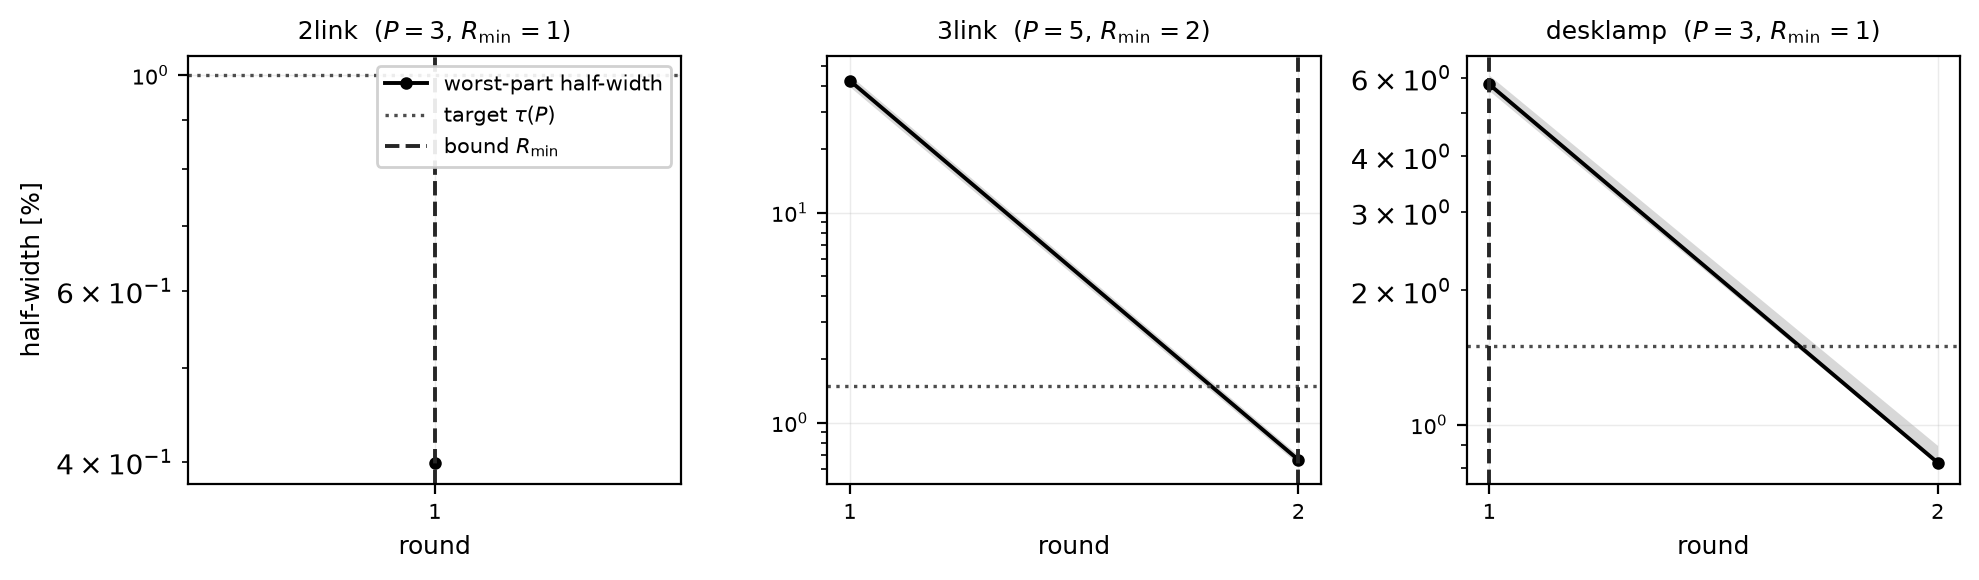
\includegraphics[width=0.74\textwidth]{fig_conv.png}
\caption{Worst-part reported half-width per round (median and interquartile
range, eight seeds). Dashed: round bound $R_{\min}$ of
Prop.~\ref{prop:rounds}; dotted: target $\tau(P)$.}
% [번역] 라운드에 대한 부위 최악 보고 반폭(seed 8개 중앙값·사분위 범위).
%   파선은 명제 3의 라운드 하한 R_min, 점선은 목표 tau(P). ("형상만으로
%   계산"은 서론·표 I 각주·IV-C 산문, "하한 등호 달성"은 IV-C 산문에.)
\label{fig:conv}
\end{figure*}

% Table 3 (main) — per-part density identification.
%   GT V/M/rho: gt.json (권위 있는 정본).  vision 열: tables/table_main_v2.tex 의
%   frozen 값을 그대로 옮김 (재채점 금지).  uniform/single/WLS/ours:
%   my_work/figures/v2/main_real.json (seeds=8, rel=5%), part별 상대 밀도오차 중앙값.
%   coverage 블록: 같은 JSON 의 95% 구간 경험적 커버리지.
%   laptop: 자산 준비 중 → 8-페이지 압축에서 행 2개를 각주 한 문장으로 이전
%   (GT·vision 수치 전부 각주에 보존, 원행은 CUTS.md).
\begin{table*}[!t]
\caption{Part-wise density identification (simulation). Ground-truth $V$, $M$,
$\rho=M/V$; method columns give the relative per-part density error [\%] (median
over eight seeds for interaction methods), lowest per row in bold.}
% [번역] 부위별 밀도 식별(시뮬레이션). 참값 V, M, rho = M/V. 방법 열은 부위별
%   상대 밀도오차 [%](상호작용 방법은 8시드 중앙값), 행별 최저는 굵게.
%   (밀도오차=질량오차 1.7e-16 불변성과 커버리지 블록 설명은 각주로 이동.)
\label{tab:main}
\centering
\scriptsize
\setlength{\tabcolsep}{4pt}
\begin{tabular}{llrrrrrrrrrr}
\toprule
& & \multicolumn{3}{c}{Ground truth} & \multicolumn{3}{c}{Vision baselines} & \multicolumn{4}{c}{Interaction (median over 8 seeds)} \\
\cmidrule(lr){3-5}\cmidrule(lr){6-8}\cmidrule(lr){9-12}
Object & Part & $V$ [cm$^3$] & $M$ [g] & $\rho$ [g/cm$^3$] & PUGS$^{\mathrm S}$ & SiPhy & \shortstack{PhysX-\\Omni} & Uniform & Single & WLS & Ours \\
\midrule
\multirow{3}{*}{Stand lamp}
 & Base    & 273.00 & 399.00 & 1.462 & 164.1 & 38.3 & 69.1  & 7.33  & 0.12 & 0.12 & \textbf{0.01} \\
 & Support &  84.50 &  85.00 & 1.006 & 10.7  & 27.3 & 183.1 & 34.64 & 1.49 & 1.27 & \textbf{0.23} \\
 & Head    &  64.10 &  87.00 & 1.357 & 36.4  & 48.5 & 58.0  & 0.21  & 0.73 & 0.55 & \textbf{0.08} \\
\midrule
\multirow{3}{*}{2-link$^{*}$}
 & Long                    & 135.72 & 49.00 & 0.361 & 7887.4 & 593.4 & \NA & 49.14 & \textbf{0.18} & 0.21 & \textbf{0.18} \\
 & Short                   & 108.12 & 42.00 & 0.389 & 7323.6 & 544.5 & \NA & 25.43 & \textbf{0.06} & 0.10 & \textbf{0.06} \\
 & Hinge$^{\mathrm h}$     &   7.45 & 41.00 & 5.506 & 423.8  & 54.5  & \NA & 51.22 & \textbf{0.34} & 0.35 & \textbf{0.34} \\
\midrule
\multirow{5}{*}{3-link$^{*}$}
 & Link 0                  & 288.12 & 100.00 & 0.347 & 4312.5 & 349.6 & \NA & 43.32  & 0.11 & \textbf{0.01} & \textbf{0.01} \\
 & Link 1                  & 208.40 &  92.00 & 0.442 & 3369.1 & 253.5 & \NA & 110.52 & 1.14 & 0.31 & \textbf{0.06} \\
 & Link 2                  & 162.28 &  69.00 & 0.425 & 3501.8 & 267.0 & \NA & 321.04 & 1.58 & 0.48 & \textbf{0.10} \\
 & Hinge 1$^{\mathrm h}$   &   7.45 &  41.00 & 5.506 & \multirow{2}{*}{178.2$^{\ddagger}$} & \multirow{2}{*}{71.7$^{\ddagger}$} & \NA & 46.45 & 0.08 & \textbf{0.04} & \textbf{0.04} \\
 & Hinge 2$^{\mathrm h}$   &   7.45 &  41.00 & 5.506 &  &  & \NA & 46.45 & 0.08 & \textbf{0.05} & 0.06 \\
\midrule
\multicolumn{5}{l}{\emph{Coverage of the reported $95\%$ interval}} & & & & & & & \\
\multicolumn{5}{l}{\quad Stand lamp} & \NA & \NA & \NA & \NA & 24/24 & 4/24  & 22/24 \\
\multicolumn{5}{l}{\quad 2-link}     & \NA & \NA & \NA & \NA & 16/16 & 14/16 & 16/16 \\
\multicolumn{5}{l}{\quad 3-link}     & \NA & \NA & \NA & \NA & 24/24 & 15/24 & 24/24 \\
\bottomrule
\end{tabular}
\vspace{2pt}
\parbox{\textwidth}{\scriptsize \textit{All methods share the same fixed part
volumes, so density error and mass error are the same number (maximum observed
difference $1.7\times10^{-16}$) and a single column reports both. The bottom block
counts, over all part--seed pairs, how often each method's reported $95\%$ interval
covers the truth. $^{\mathrm h}$ hinge modelled as its own
unknown. $^{\mathrm S}$ Stand-lamp PUGS masses integrate its frozen SAM-partitioned
Gaussian volume and point-wise density, scored at the midpoint of its predicted mass
range; other PUGS rows and all SiPhy rows distribute each object-level prediction
using ground-truth volume fractions (Sec.~\ref{sec:setup}). PhysX-Omni is N/A where
its generated shape admits no canonical part mapping. $^{\ddagger}$ vision baselines
were scored on the two hinges jointly. $^{*}$ preliminary pre-ballast custom-object
masses and densities; CAD volumes are fixed. On the 2-link object Ours and Single
are byte-identical (Sec.~\ref{sec:sim}). Single's intervals
cover only because they are wide (Sec.~\ref{sec:sim}), and its convergence flag
never consults the stopping rule.
The fourth object, the laptop (display\,/\,base: $V=354.10/798.60\,
\mathrm{cm^3}$, $M=379.25/1137.75\,\mathrm{g}$, $\rho=1.071/1.425\,\mathrm{g/cm^3}$;
vision errors PUGS $76.7/30.1$, SiPhy $182.5/108.0$, PhysX-Omni $417.3/611.8\,\%$),
contributes ground-truth and vision-baseline data only: \rev{its mesh and URDF are
in preparation, so all its interaction columns are pending}.}}
\end{table*}



Each object runs the closed loop over eight seeds ($5\%$ joint-angle error,
$\tau=0.5\%\times P$); Table~\ref{tab:main} is the main result.
Prop.~\ref{prop:rounds} reads off geometry (Table~\ref{tab:objects}): the
3-link object's five unknowns exceed the rank-four ceiling, so a second
configuration is \emph{necessary} before any wrench is simulated.
% [번역] 각 물체는 각도오차 5 %, tau = 0.5 % x P 로 여덟 시드 폐루프를 돌며
%   표 III 이 메인 결과다. 명제 3은 형상만으로 읽힌다(표 I): 3링크는
%   미지수 다섯이 rank 4 천장을 넘어 렌치 시뮬 전에 이미 두 번째 형상이
%   '필요' 하다.

The loop meets that bound (one round on the 2-link object, two elsewhere;
all seeds converge). Uniform fails by orders of magnitude: the mass redistributions it misses
stay invisible to shape until a second articulation configuration
(Prop.~\ref{prop:null}).
% [번역] 루프는 그 하한대로 2링크 한 라운드, 나머지 두 라운드에 끝나고 전
%   시드 수렴한다. uniform 은 자릿수로 틀린다 — 놓친 질량 재분배는 두 번째
%   관절 형상 전까지 형상에 안 보인다(명제 2).

On the 2-link
object \emph{ours is single}: three unknowns fit under the rank-four
ceiling, and the two columns of Table~\ref{tab:main} are
byte-identical---the positive direction of Prop.~\ref{prop:rounds}, not a
win; only uniform is separated there. Single's failure appears on the 3-link
object, in the half-width rather than the point error: its worst-part error
is a respectable $1.58\%$, but its half-widths for the three links are
$2.6$, $28.7$, and $42.5\%$---one configuration cannot \emph{certify} five
unknowns.
% [번역] 2링크에서는 'ours 가 곧
%   single' — 미지수 셋이 rank 4 천장 아래라 표 III 두 열은 바이트 단위로
%   같다. 명제 3의 양의 방향이지 승리가 아니며 갈리는 것은 uniform 뿐.
%   single 의 실패는 3링크에서, 점오차 아닌 반폭에서다 — 최악 part 오차
%   1.58 % 는 준수하나 세 링크 반폭이 2.6 / 28.7 / 42.5 %: 형상 하나로
%   미지수 다섯을 '증명' 못 한다. (수렴 플래그가 무의미하다는 것과 single 의
%   커버리지가 폭 때문이라는 것은 표 III 각주가 싣는다.)

The strongest ablation evidence is the coverage block of
Table~\ref{tab:main}. WLS shares our loop, ignoring only the
errors-in-variables structure; its point errors stay within an order of
magnitude of ours, but its $95\%$ intervals miss the truth on up to $20$ of
$24$ part--seed pairs where ours cover at target width: the bias
Eq.~\eqref{eq:tls} removes does not shrink with rounds. Single's coverage
comes only from width. An estimator feeding a simulator must know when it
is wrong.
% [번역] 가장 강한 ablation 근거는 표 III 커버리지 블록이다. 루프를 공유하고
%   EIV 구조만 무시하는 WLS 는 점오차는 한 자릿수 안이지만 95 % 구간이
%   최대 24쌍 중 20쌍에서 참값을 놓친다(우리는 목표 폭으로 커버; 개별 수치는
%   표 III) — 식 (7) 이 제거하는 편향은 라운드를 쌓아도 안 준다. single 의
%   커버리지는 오직 폭 덕분이다. 시뮬레이터에 밀도를 넘길 추정기는 제가 틀린
%   때를 알아야 한다.

The hinge rows are the built-for case: densities recovered to $0.04$--$0.34\%$, intervals covering on all seeds, at
$3.0$--$3.8\%$ half-widths honestly reflecting the occluded part's weaker
observability. The stand lamp has no hinge body, so this rests on the custom
objects only.
% [번역] 힌지 행이 커스텀 물체를 만든 이유다. 밀도 0.04~0.34 %
%   복원, 구간은 전 시드에서 덮고, 반폭 3.0~3.8 % 는 가려진 part 의 약한
%   관측성을 정직하게 반영한다. 램프에는 힌지 body 가 없어 커스텀 둘에만
%   근거한다.

The stand lamp attains full rank in one configuration yet runs two: past
full rank, conditioning governs, set by joint-angle precision rather than
rank (Remark~\ref{rem:cond}, Fig.~\ref{fig:conv}).
% [번역] 램프는 형상 하나에서 full rank 인데 두 라운드를 돈다. full rank
%   이후는 조건수가 지배하고, 그것은 rank 아닌 각도 정밀도가 만든다
%   (Remark 3, 그림 5).

Synthetic chains of $P{=}2\ldots6$ unknowns separate the methods cleanly.
Through $P=3$ everything but uniform suffices; from $P=4$ the rank-four
ceiling of Cor.~\ref{cor:rigid} appears directly in \emph{single}, whose
worst-part error climbs $17.06\to32.02\to53.57\%$ as $P$ grows past four,
while WLS degrades $10.53\to11.79\to21.39\%$ and ours stays below $0.6\%$
throughout. At $P=4$ ours converges in a median of
$3$ rounds where offline D-optimal
design~\cite{gautier1992exciting,swevers1997optimal} needs $4$ and random
selection needs $21$ and fails once in eight; at $P=5$ the gap widens to $7$
against $10$ and random never converges ($0/8$). All three share the
criterion, so closed-loop re-selection is the only difference.
\rev{The $P=6$ arm is still computing.} Beyond $P=5$, though, no criterion---D, A, or E---reaches a $1\%$ target in
twelve rounds: at $\pm5\%$ angular error the binding resource is angular
precision, not the criterion.
% [번역] 미지수 P = 2..6 합성 사슬이 방법들을 깨끗하게 가른다. P <= 3 은 uniform
%   빼고 전부 충분하다. P = 4 부터 따름정리 2의 rank 4 천장이 single 에 그대로
%   나타나, 부위 최악 오차가 P 가 4를 넘어가며 17.06 -> 32.02 -> 53.57 % 로 오른다.
%   WLS 는 10.53 -> 11.79 -> 21.39 %, 우리는 전 구간 0.6 % 미만(0.25, 0.51, 0.59 %).
%   P = 4 에서 우리는 라운드 중앙값 3 으로 수렴하는데 고전 오프라인 D-최적 설계는 4,
%   무작위 선택은 21 이 필요하고 8회 중 1회는 실패한다. P = 5 에서는 격차가
%   7 대 10 으로 벌어지고 무작위는 예산 안에 아예 수렴하지 못한다(0/8).
%   셋이 기준을 공유하므로 차이는 폐루프 재선택 그 자체다. P = 6 arm 은 계산 중.
%   다만 기준 선택이 이 영역을 구제하지는 못한다 — P = 5 부터는 D, A, E 어느
%   기준도 12라운드 안에 목표 1% 에 닿지 못한다. 각도오차 ±5% 에서는 그만큼의
%   미지수를 가를 정보가 측정에 애초에 없기 때문이다. 구속하는 자원은 기준이
%   아니라 각도 정밀도다.



\subsection{Measurement Pose and Path Design}
\label{sec:posepath}

\begin{figure*}[!t]
\centering
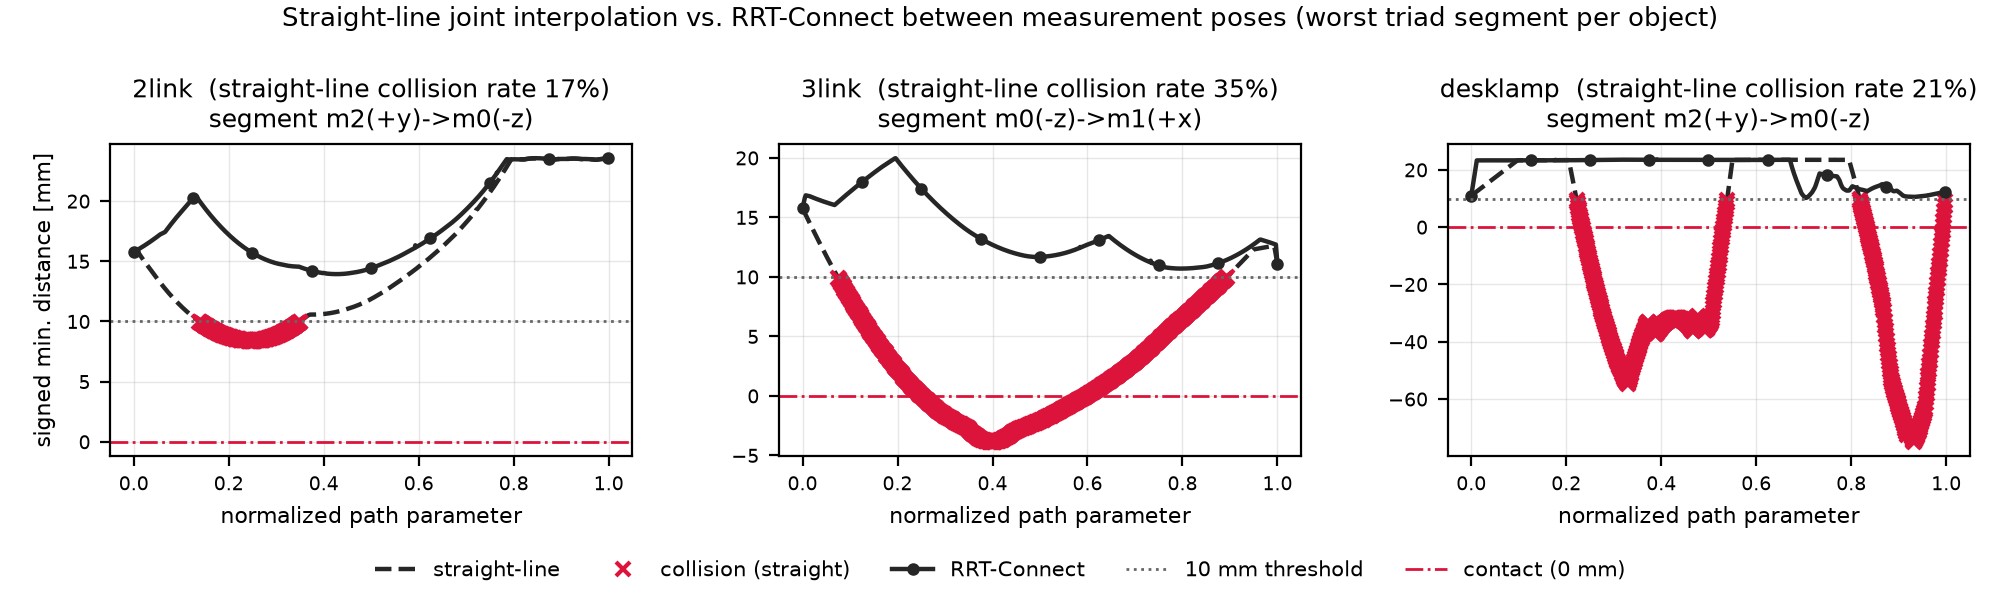
\includegraphics[width=0.74\textwidth]{fig_path.png}
\caption{One row per object at its most informative colliding
configuration: joint-space paths, minimum clearance (dashed: straight;
solid: RRT-Connect), and end-link workspace trace.}
% [메모] Fig. 6 — 파일: figures/v2/fig_path.png.
\label{fig:path}
\end{figure*}

% Table 4 — 경로 비교 (figures/v2/path_compare.json 'all' 범위).
%   구 panel (a)(중력 방향 수확체감, study_tilt.py 실측)는 8-페이지 압축에서
%   삭제 — 수치는 IV-D 산문에 흡수, 원문은 CUTS.md.  E4b 주의 4건 반영:
%   관절한계 열은 두 계획기 모두 구조적으로 0 (볼록 상자) — 승리로 쓰지 말 것.
%   밀도오차 열: 두 계획기는 같은 측정 자세를 이으므로 추정치는 동일 —
%   각주로 설명 (숫자를 지어내지 않는다).
\begin{table}[!htb]
\caption{Straight-line joint interpolation vs.\ RRT-Connect over every pose pair
of the configuration grid (each cell: straight\,/\,RRT-Connect), with
per-configuration information gain $\Delta I$ and whitened-regressor condition
number $\kappa$.}
% [번역] 전체 형상 격자의 모든 자세쌍에서 직선 보간 대 RRT-Connect(칸마다
%   직선/RRT-Connect), 형상별 정보이득 Delta I 와 백색화 회귀행렬 조건수
%   kappa. (두 계획기의 밀도 추정 동일 문장은 각주로 이동.)
\label{tab:path}
\centering
\scriptsize
\setlength{\tabcolsep}{3pt}
\begin{tabular}{lccccc}
\toprule
Object & \shortstack{$\Delta I$ [nat] /\\cond.\ $\kappa$} & \shortstack{Coll.\\{[\%]}} & \shortstack{Pen.\\{[mm]}} & \shortstack{Clear.\\{[mm]}} & \shortstack{Time\\{[s]}} \\
\midrule
2-link & \shortstack{4.0--4.5\\57--324} & 25.0\,/\,\textbf{0.0} & 83.5\,/\,\textbf{0.0} & 0.6\,/\,13.1 & $\sim$0\,/\,0.12 \\
\addlinespace[2pt]
3-link & \shortstack{6.3--11.1\\$10^{16}$--$10^{18}$} & 20.9\,/\,\textbf{0.0} & 33.1\,/\,\textbf{0.0} & 11.3\,/\,14.1 & $\sim$0\,/\,0.11 \\
\addlinespace[2pt]
Stand lamp & \shortstack{6.9--9.3\\8.9--100} & 21.1\,/\,\textbf{0.0} & 93.8\,/\,\textbf{0.0} & $-0.8$\,/\,12.0 & $\sim$0\,/\,0.43 \\
\bottomrule
\end{tabular}
\vspace{2pt}
\parbox{\linewidth}{\footnotesize \textit{Coll.\ = fraction of pose pairs whose path
touches an obstacle; Pen.\ = maximum penetration depth; Clear.\ = mean minimum
clearance (negative = inside an obstacle on average); Time = mean planning time per
pair. Both planners connect the same measurement poses, so the wrench data and
hence the density estimate (Table~\ref{tab:main}) are unchanged; what differs is
whether the path is executable without contact. Joint-limit violations are zero for both planners by construction
(Sec.~\ref{sec:posepath}). The 3-link condition numbers are structural, not
numerical: one configuration observes total mass and first moment (rank $4$)
against five unknowns, the rank-four ceiling of Prop.~\ref{prop:rank} appearing
directly in the conditioning; the two three-unknown objects are full rank.}}
\end{table}



How many gravity directions per round: two orthogonal directions reach the
rank ceiling, and the orthonormal triad is the knee of diminishing
returns---$12.88$ nat for one direction, $25.41$ for two, $26.35$ for the
triad, only $27.73$ for six---while one direction is anisotropic
($2.72\times$): a gravity-aligned joint axis hides distal mass.
% [번역] 라운드당 중력 방향 개수: 직교 2방향이면 rank 천장에 닿고 직교정규
%   삼면체가 수확체감의 꺾이는 지점이다 — 1방향 12.88 nat, 2방향 25.41,
%   삼면체 26.35, 6방향이라야 27.73 — 단일 방향은 비등방적이다(배향 따라
%   2.72배): 중력과 나란한 관절 축이 그 아래 질량을 숨긴다.

The triad's free $SO(3)$ orientation (Cor.~\ref{cor:invariance}) is spent on
the joints: rotating it to minimize peak torque on those joints preserves
the information \emph{exactly}---$26.3535$ nat before and
after, a $0.0\%$ loss---while cutting peak joint torque from $1.031$ to
$0.620\,\mathrm{N\cdot m}$, a $39.9\%$ reduction: the quantitative basis for
claiming measurement does not endanger the object's joints.
% [번역] 삼면체의 공짜 SO(3) 방향(따름정리 1)은 관절 보호에 쓴다. 그 관절의
%   최대 토크를 최소화하도록 돌리면 정보는 '정확히' 보존되고 — 전후 26.3535
%   nat, 손실 0.0 % — 최대 관절 토크는 1.031 → 0.620 N·m, 39.9 % 감소다.
%   측정이 물체의 관절을 상하게 하지 않는다는 주장의 정량적 근거다.

We grid each joint range at five values, plan every pose pair (triad cycles,
home transits), and score straight-line interpolation against RRT-Connect
(Table~\ref{tab:path}, Fig.~\ref{fig:path}); RRT-Connect never collides, at
negligible path-length and planning-time cost.
% [번역] 관절당 다섯 값 격자의 모든 자세쌍(삼면체 순환, home transit)을
%   계획해 직선 보간 대 RRT-Connect 를 채점한다(표 IV, 그림 6). RRT-Connect
%   는 무충돌 — 경로·계획시간 비용은 무시할 만하다.

The worst \emph{table} penetration is
$33.1\,\mathrm{mm}$ (3-link tip link), while the larger $93.8$ and
$83.5\,\mathrm{mm}$ figures are the object penetrating the robot's own wrist
and forearm. Joint-limit violations are zero for \emph{both} planners, necessarily (the
limits form a convex box): interpolation fails by collision, never by limit
violation. Nor always---the 3-link transits are straight-line
collision-free---so feasibility is re-checked per configuration.
% [번역] 최악 '테이블' 관통은 33.1 mm(3링크 끝 링크), 더 큰 93.8 / 83.5 mm
%   는 물체가 로봇 손목·전완에 파고드는 관통이다. 관절한계 위반은 '두'
%   계획기 모두 0 이며 필연이다(한계는 볼록 상자): 직선 보간의 실패 방식은
%   충돌이지 한계 위반이 아니고, 항상 실패하지도 않는다 — 3링크 transit 은
%   직선도 무충돌이라 실현가능성은 형상마다 재검사한다.



\subsection{Sim-Ready Asset Validation}
\label{sec:asset}

\begin{figure*}[!t]
\centering
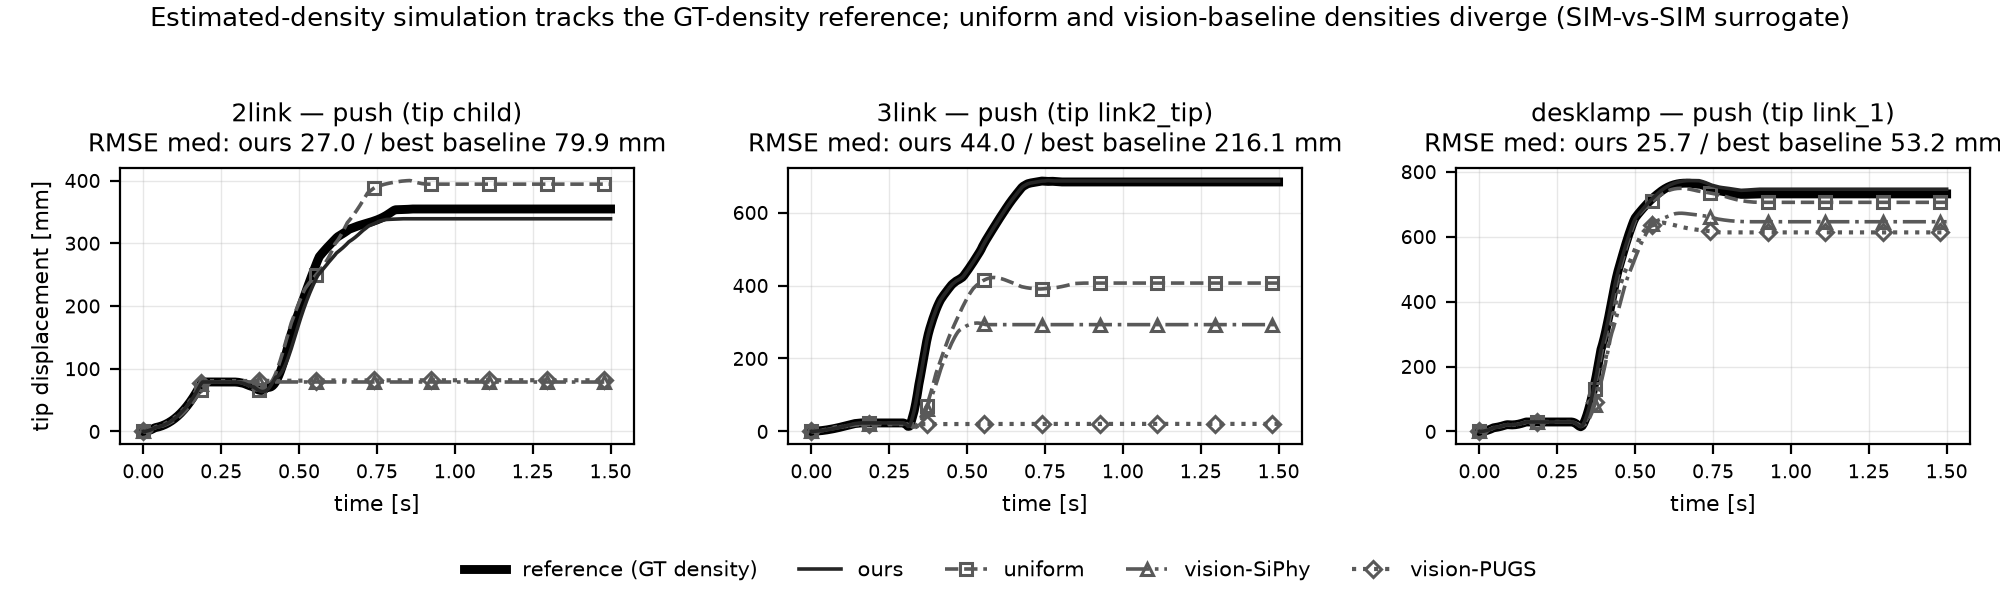
\includegraphics[width=0.74\textwidth]{fig_asset.png}
\caption{Asset dynamic fidelity (\emph{simulation-only surrogate}): tip
displacement in three scenarios against the ground-truth-density reference
plant. \rev{[Sim-vs-real version awaits the hardware sessions.]}}
% [번역] asset 동적 충실도(시뮬 전용 대리 검증): 세 시나리오의 끝단 변위를
%   참값 밀도 기준 plant 와 비교. sim-vs-real 판은 하드웨어 세션 대기.
%   ("밀도만 다름"과 2링크 release 둔감성은 IV-E 산문에.)
% [메모] Fig. 7 — 시뮬 대리 검증 그림(figures/v2/fig_asset.png).  구 Fig. 8
%   (실물 비교 자리표시자)은 이 캡션의 rev 로 흡수, fig:assetreal 라벨 보존.
\label{fig:asset}
\label{fig:assetreal}
\end{figure*}

% Table 5 — sim-ready asset 검증.  출처: figures/v2/asset_validation.json (E5).
%   ★ 시뮬-시뮬 대리 검증: reference 는 GT-밀도 plant 이지 현실이 아니다.
%   캡션·헤더에 명시.  8-페이지 압축: 9행 -> push 3행 (Fig. 7 시나리오와 일치),
%   release·drop 순서는 본문 한 문장, 원행은 CUTS.md.  2link release 구조적
%   둔감 서술은 본문 산문에 잔존.  개입/시간 블록: 가이드라인 요구.
%   실물 타이밍은 \Pending.
\begin{table}[!htb]
\caption{Sim-ready asset validation, a \emph{simulation-only surrogate}:
median worst-part trajectory RMSE [mm] against the ground-truth-density
reference plant, \textsc{push} scenario of Fig.~\ref{fig:asset}, with the
user intervention each asset requires.}
% [번역] sim-ready asset 검증(시뮬 전용 대리 검증): 참값 밀도 기준 plant 대비
%   최악 part 궤적 RMSE [mm] 중앙값, 그림 7의 push 시나리오, 아래 블록은
%   asset 별 사용자 개입. (공유 상수·초기조건 5개·release/drop 요약은 각주와
%   IV-E 산문으로 이동.)
\label{tab:asset}
\centering
\scriptsize
\setlength{\tabcolsep}{3pt}
\begin{tabular}{lrrrr}
\toprule
& \multicolumn{4}{c}{\shortstack{Worst-part RMSE [mm], \textsc{push}\\vs.\ GT-density plant (simulation)}} \\
\cmidrule(lr){2-5}
Object & Ours & Uniform & SiPhy & PUGS \\
\midrule
2-link     & \textbf{26.97} & 79.94  & 338.68 & 342.36 \\
3-link     & \textbf{43.97} & 216.13 & 491.38 & 582.44 \\
Stand lamp & \textbf{25.66} & 53.16  & 325.22 & 363.97 \\
\midrule
\multicolumn{4}{l}{\emph{User intervention}} & Time \\
\multicolumn{1}{l}{\quad Ours}
 & \multicolumn{3}{l}{as RORA $+$ scale $+$ joint adj.\ (1--2$\times$)} & \Pending \\
\multicolumn{1}{l}{\quad Uniform}
 & \multicolumn{3}{l}{as RORA $+$ scale; no interaction} & \Pending \\
\multicolumn{1}{l}{\quad SiPhy}
 & \multicolumn{3}{l}{single RGB image; no interaction} & \Pending \\
\multicolumn{1}{l}{\quad PUGS}
 & \multicolumn{3}{l}{multi-view scan; no interaction} & \Pending \\
\bottomrule
\end{tabular}
\vspace{2pt}
\parbox{\linewidth}{\footnotesize \textit{The reference is a plant carrying the
ground-truth densities, \emph{not} the real object; contact stiffness,
dissipation, friction, and joint damping are shared constants across all
variants, so only the per-part densities differ. Medians are over five
pre-registered initial conditions; release and drop are summarized in the text
(Sec.~\ref{sec:asset}). \rev{End-to-end wall-clock time requires the hardware
runs and is pending.} Vision-baseline densities carry the
relative errors of Table~\ref{tab:main} with an assumed positive sign; PhysX-Omni
is excluded because it is N/A on both custom objects.}}
\end{table}



This validation is a \emph{simulation-only surrogate}: the reference is a
Drake plant carrying the ground-truth densities, not the real object, and
nothing here is a real-world claim. \rev{The sim-to-real comparison
(Fig.~\ref{fig:assetreal}) requires the hardware sessions and is pending.}
Contact, friction, and damping parameters are shared constants, so the
comparison isolates exactly what we identify: the per-part densities.
% [번역] 이 검증은 '시뮬레이션 전용 대리 검증' 이다. 기준은 참값 밀도를
%   실은 Drake plant 이지 실제 물체가 아니고, 여기의 어떤 것도 실세계 주장이
%   아니다. sim-to-real 비교(그림 7 내 rev)는 하드웨어 세션 대기로 pending.
%   접촉·마찰·댐핑 계수는 공유 상수 — 우리 식별 대상이 아니다 — 라 비교는
%   부위별 밀도만 격리한다.

Each variant runs release, drop, and push; ours ranks first in all $27$
scenario cells. Table~\ref{tab:asset} reports the push rows matching
Fig.~\ref{fig:asset}; release and drop preserve the same ordering at larger
margins---orders of magnitude, versus $2.1$--$14.2\times$ on push, where
contact amplifies every variant's error, ours included: a ranking, not
absolute accuracy.
% [번역] 각 asset 변형을 release·drop·push 로 구동해 최악 part 궤적 RMSE 로
%   판정하며, 27개 시나리오 칸 전부에서 우리가 1위다. 표 V 는 그림 7과 같은
%   push 행만 싣고, release·drop 은 같은 순서를 더 큰 격차로 보존한다 — 수
%   자릿수 대, 접촉이 모든 변형의 오차를 증폭하는 push 의 2.1~14.2배: push 는
%   절대 정확도가 아니라 순위다.

The 2-link release must not be over-read: it is structurally blind to
density---with the root link welded, the single pendulum's motion is
invariant to scaling the moving link's density, so its sub-millimetre RMSE
reflects that invariance, not skill---and release trajectories
settle onto joint limits, under-stating differences.
% [번역] 2링크 release 는 과대 해석 금지. 구조적으로 밀도에 눈멀어 있다 —
%   뿌리 링크를 용접하면 단진자라 움직이는 링크의 밀도 배율에 불변, sub-mm
%   수치는 실력이 아니라 그 불변성이다 — release 는 관절 한계에 내려앉아
%   차이를 과소평가한다. (vision 변형의 양의 부호 가정은 표 V 각주.)

Intervention is part of the asset's specification (Table~\ref{tab:asset}):
the addition over the inherited RORA~\cite{lee2026rora} stage is the joint
adjustment, once per round---one to two rounds here \rev{(operator and
wall-clock times await the hardware sessions)}.
% [번역] 개입은 asset 사양의 일부다(표 V). 상속되는 RORA 단계 위에 추가되는
%   것은 joint 조정뿐, 라운드당 한 번 — 여기서는 한두 라운드다(작업자·전체
%   소요 시간은 하드웨어 세션 대기).



% [메모] 8/30 v2 개정 (가이드라인 [Conclusion] 3단락 + WRITING_BRIEF §4,8,9).
%   1단락 문제·제안, 2단락 실측 요약(시뮬 3물체 — laptop/실물은 \rev),
%   3단락 limitation: 채택 요소 3개 + 실험이 드러낸 2개(부피 오차의 조건수
%   비용, 관성 텐서 비식별) + future work(관절각 dynamics, RPNA).
\section{Conclusion}

A sim-ready articulated asset requires per-part volume \emph{and} density;
vision-based estimation is inaccurate, and interaction-based identification
rigid-only. PIVoT identifies per-part density in a closed loop:
information-gain joint-configuration selection, three gravity-direction
measurement poses linked by collision-free paths, and uncertainty-aware
updates.
% [번역] 관절 물체의 sim-ready asset 에는 part 별 부피'와' 밀도가 모두
%   필요한데, 비전 기반 추정은 부정확하고 상호작용 기반 식별은 강체에
%   국한되어 왔다. 우리는 정보이득 기반 관절 형상 선택, 서로 다른 중력 방향의
%   측정 자세 3개와 그 사이 collision-free 경로, 불확실성 기반 밀도 갱신으로
%   구성된, part 별 밀도를 능동 상호작용으로 식별하는 폐루프 파이프라인
%   PIVoT 를 제시했다.

On three simulated objects, worst-part density error was 0.18, 0.11, and
0.23\%, versus a homogeneous baseline's 49.1, 321.0, and 34.6\%. Stronger
evidence is the interval: our 95\% intervals covered the truth in 62 of 64
part--seed pairs, a WLS ablation in only 33 of 64---the errors-in-variables
bias does not shrink with rounds, and a WLS interval cannot see it---and a
single configuration cannot certify five unknowns, its half-widths reaching
42.5\% (Cor.~\ref{cor:rigid}). Omitting the custom objects' friction hinge
as its own unknown yields a 79.1\% hinge error under a claimed 0.83\%
half-width. The intervention added for physics estimation is one
joint-configuration adjustment; the reconstruction-stage intervention is
inherited from \cite{lee2026rora}. \rev{Validation on the laptop asset and
the physical robot is in preparation.}
% [번역] 시뮬레이션 3개 물체에서 최악 part 의 상대 밀도 오차는 0.18, 0.11,
%   0.23\% 로, 균일밀도 baseline 의 49.1, 321.0, 34.6\% 와 대비된다. 더 강한
%   근거는 구간이다. 우리의 95\% 구간은 64개 부위-시드 쌍 중 62를 덮었고
%   WLS ablation 은 33에 그쳤다 — errors-in-variables 치우침은 라운드를
%   늘려도 줄지 않고, WLS 구간은 그것을 보지 못한다 — 단일 형상은 미지수
%   다섯을 증명하지 못해 반폭이 42.5\% 에 이른다(따름정리). 마찰 힌지를 독립
%   미지수로 두지 않으면 반폭 0.83\% 를 주장하면서 힌지 오차 79.1\% 를 낸다.
%   물성 추정을 위해 추가되는 개입은 관절 형상 조정 한 번이며, 재구성 단계의
%   개입은 [RORA] 에서 상속된다. (laptop 자산과 실물 로봇 검증은 준비 중 —
%   \rev{} 표시.)

Limitations begin with adopted components: the input reconstruction's
segmentation and joint errors propagate downstream, with its
human-in-the-loop intervention \cite{lee2026rora}; sampling-based RRT grows
costly on complex topologies without optimality guarantees; and a single
linkage gripper on a 6-DoF arm restricts validation to small, light
objects. The experiments add two. Volume error is not benign: density error tracks
it one-to-one, inertia as $s^2$ (Rem.~\ref{rem:volume}), part mass is far
less sensitive yet not exactly invariant, and it multiplies rounds
(Sec.~\ref{sec:vol})---the practical limit is conditioning, set by volume
and joint-angle precision, not rank. The inertia tensor is not identified: the quasi-static
wrench never sees it, so we derive it from mesh geometry and
identified density, inheriting mesh scale error quadratically. Future work: estimate joint-angle dynamics and reorient accordingly, where
tools like RPNA~\cite{wensing2024geometric} become
discriminative.
% [번역] 한계는 먼저 채택한 구성 요소에서 온다. 입력 재구성의 part
%   segmentation 과 관절 추정 오류는 human-in-the-loop 개입과 함께 이후
%   단계로 상속되고 [RORA], 샘플링 기반 RRT 는 복잡한 topology 에서 계산이
%   늘며 최적성을 보장하지 않고, 단일 linkage gripper 와 6자유도 팔은 검증
%   대상을 소형·경량 물체로 좁힌다. 실험은 둘을 더한다. 부피 오차는 무해하지
%   않다. 밀도 오차는 이를 1:1 로, 관성은 s^2 로 따라가고(비고), part 질량은
%   훨씬 덜 민감하지만 엄밀히 불변은 아니며, 라운드 수를 곱으로 늘린다
%   (IV-B: 1→7, 3/8 미수렴). 즉 실질적 한계는 rank 가 아니라 부피·관절각
%   정밀도가 정하는 조건수다. 또한 관성 텐서는 식별되지 않는다. 준정적 회전 방정식에서
%   사라지므로 메시 기하와 식별된 밀도에서 유도하며, 메시 배율 오차를 제곱으로
%   물려받는다. Future work 는 관절각 dynamics 를 추정해 그에 맞춰 물체를
%   재배향하는 것이며, 거기서는 RPNA 같은 도구가 실제 판정력을 갖는다.


\section*{Acknowledgment}
% TODO: Acknowledgment 작성

\begingroup
\hbadness=2000
\bibliographystyle{IEEEtran}
\bibliography{reference}
\endgroup

\end{document}
